% Self-contained draft: bibliography and vector figures included.
\documentclass[11pt]{article}
% Begin preamble
\usepackage[T1]{fontenc}
\usepackage[utf8]{inputenc}
\usepackage{lmodern}
\usepackage[margin=1in]{geometry}
\usepackage{amsmath,amssymb,amsthm,mathtools}
\usepackage{booktabs,tabularx,array,enumitem,microtype}
\usepackage{needspace}
\usepackage[dvipsnames]{xcolor}
\usepackage{tikz}
\usetikzlibrary{arrows.meta,positioning}
\usepackage{graphicx}
\usepackage[colorlinks=true,linkcolor=MidnightBlue,citecolor=MidnightBlue,
urlcolor=MidnightBlue,pdftitle={Exact Reference-Assisted Entropy Contraction from the Choi Matrix},
pdfauthor={Harjas Sandhu}]{hyperref}
\usepackage[nameinlink,noabbrev]{cleveref}
\numberwithin{equation}{section}
\newtheorem{theorem}{Theorem}[section]
\newtheorem{lemma}[theorem]{Lemma}
\newtheorem{proposition}[theorem]{Proposition}
\newtheorem{corollary}[theorem]{Corollary}
\theoremstyle{definition}
\newtheorem{definition}[theorem]{Definition}
\newtheorem{example}[theorem]{Example}
\theoremstyle{remark}
\newtheorem{remark}[theorem]{Remark}
\DeclareMathOperator{\Tr}{Tr}
\DeclareMathOperator{\ran}{ran}
\DeclareMathOperator{\supp}{supp}
\DeclareMathOperator{\id}{id}
\DeclareMathOperator{\Rea}{Re}
\DeclareMathOperator{\Ad}{Ad}
\DeclareMathOperator{\diag}{diag}
\DeclareMathOperator{\rank}{rank}
\newcommand{\N}{\mathcal N}
\newcommand{\M}{\mathcal M}
\newcommand{\E}{\mathcal E}
\newcommand{\D}{\mathcal D}
\newcommand{\HS}{\mathrm{HS}}
\newcommand{\one}{\mathbf 1}
\newcommand{\ket}[1]{\lvert #1\rangle}
\newcommand{\bra}[1]{\langle #1\rvert}
\newcommand{\ip}[2]{\langle #1,#2\rangle}
\newcommand{\norm}[1]{\lVert #1\rVert}
\newcommand{\etaC}{\eta_D^{\mathrm c}}
\newcommand{\etaDel}{\eta_D^{\Delta}}
\newcommand{\etaCM}{\eta_{\mathrm{condMI}}}
\newcommand{\etaMI}{\eta_{\mathrm{MI}}}
\newcommand{\etaOrd}{\eta_D^{\mathrm{ord}}}
\newcommand{\etaP}{\eta_D^{\mathrm{prod}}}
\newcommand{\cov}{\mathsf C}
\newcommand{\States}{\mathsf D}
\newcommand{\BKM}{\mathrm{BKM}}
\newcommand{\SLD}{\mathrm{SLD}}
\newcommand{\dd}{\,\mathrm d}
\newcolumntype{Y}{>{\raggedright\arraybackslash}X}
\setlist[enumerate]{leftmargin=*,itemsep=3pt}
\setlist[itemize]{leftmargin=*,itemsep=3pt}
\setlength{\emergencystretch}{2em}
\hypersetup{bookmarksnumbered=true}
% End preamble

\title{Exact Reference-Assisted Entropy Contraction\\from the Choi Matrix}
\author{Harjas Sandhu\\[3pt]\small The University of Queensland\\
\small\href{mailto:harjas.sandhu@student.uq.edu.au}{harjas.sandhu@student.uq.edu.au}}
\date{14 November 2026}
\begin{document}
\maketitle
\begin{abstract}
How much distinguishability can a quantum channel preserve when its input is
correlated with an untouched quantum reference? We give an exact finite
semidefinite program for the complete, equal-reference Umegaki contraction
coefficient of every finite-dimensional channel. Its value also equals the
reference-subtracted relative-entropy coefficient and the conditional
mutual-information coefficient. The program uses the unnormalized Choi matrix;
its inverse formulation requires an explicit range condition. The proof
identifies a centered complete Gram optimization, constructs a state-independent
signed observable lift through an erasure channel, and proves sharpness with a
rare coherent reference sector. References of bounded dimension suffice, even
when both input marginals are prescribed and faithful. The same program computes
the corresponding coefficients for regular modular Petz divergences, each fixed
Petz R\'enyi order between zero and one, and quantum Chernoff divergence.
Consequences include a harmonic dual, exact tensor products, a sharp comparison
with positive CP-replacer minorization, and explicit classical and unitary-noise
formulas. We separately compute ordinary quantum mutual-information contraction
for qubit depolarization, which is strictly smaller. A discontinuity at pure
reset rules out uniformly bounded-use black-box estimation, distinguishing exact
Choi-data evaluation from robust acquisition of an unknown channel.
\end{abstract}
\tableofcontents
% Begin sections/01-introduction
\section{Introduction}
\label{sec:introduction}

A noisy channel reduces the distinguishability of quantum states. Quantifying
that reduction is a basic problem in information theory, with uses in statistical
comparison, information propagation and the analysis of noisy dynamics. The
answer depends on what information is allowed outside the channel. An untouched
reference can retain information perfectly. Consequently, the unrestricted
ratio of input and output relative entropies becomes trivial if the compared
reference states may differ and that contribution is left unaccounted for.

Two established definitions avoid this problem. The \emph{complete} coefficient
compares joint states with the same reference marginal. The \emph{conditional}
coefficient instead subtracts the reference relative entropy from both numerator
and denominator. George, Hirche, Nuradha and Wilde introduce the complete
coefficient and CP-replacer bounds in their quantum Doeblin
framework~\cite[Definition~11 and Section~6.1]{GHNW26}. Hirche, George, Nuradha
and Wilde develop the conditional framework and identify its Umegaki coefficient
with conditional-mutual-information contraction~\cite[Theorem~1 and
Corollary~3]{HGNW26}. Their Section~3.3 asks how complete, conditional and ordinary
mutual-information contraction compare, including for depolarizing channels.

The main contribution here is an exact value for the complete and conditional
coefficients of an arbitrary finite channel. An optimization over references and
state pairs of unbounded dimension is replaced by one finite semidefinite
program in the channel's Choi matrix. A matching construction proves that the
program gives the coefficient itself, rather than a sufficient upper bound.
It also bounds the reference dimension needed to approach the optimum. The
complete and conditional Umegaki coefficients coincide for every channel. For
qubit depolarization, the ordinary quantum mutual-information coefficient is
strictly smaller, as shown by a separate argument.

\paragraph{Foundations and attribution.}
The proof uses established machinery in specific roles. Stinespring
factorization~\cite{Stinespring55}, Choi's representation~\cite{Choi75} and
convex minimax~\cite{Sion58} provide the finite geometry. Signed observable
lifting and the conversion of complete weighted-square inequalities into
relative-entropy comparison are developed by Zhu and
Wang~\cite[Definition~S3, Proposition~S4, Theorem~S5 and Lemmas~S2,
S6--S7]{ZW26v3}. Hirche establishes related complete estimation orders and
signed-lift characterizations~\cite[Theorem~3.2 and Proposition~3.5]{Hirche26}.
We prove the particular lifting and integration statements needed here. The
additional operations are solving the centered one-channel optimization,
reducing its complex center to a positive one, and obtaining its sharp coherent
converse.

The modular-divergence extension uses the positive integral representation of
operator-convex functions~\cite[Theorem~2.2]{FH14}. It concerns modular Petz
divergences, unlike the hockey-stick integral divergences of
Hirche and Tomamichel~\cite{HT24}. Ordinary, unreferenced contraction coefficients
can depend on the chosen divergence~\cite{HR15}. Complete entropy decay toward
a specified equilibrium or conditional expectation~\cite{GR22} is also a
different optimization. These distinctions are material, not changes of notation.

\begin{table}[htbp]
\centering\small
\begin{tabularx}{\textwidth}{@{}p{.27\textwidth}YY@{}}
\toprule
Established ingredient & Role retained here & Added conclusion \\
\midrule
Complete and conditional coefficient frameworks~\cite{GHNW26,HGNW26}
 & Definitions, reference subtraction and information interpretation
 & Exact common all-channel value and bounded-reference sharpness \\
Signed lifts and metric comparison~\cite{ZW26v3,Hirche26}
 & Statistical reconstruction without positivity of the lift
 & Optimal comparison with erasure, expressed in the Choi matrix \\
Positive-resolvent representation~\cite{FH14}
 & Integral decomposition of regular operator-convex generators
 & One exact coefficient for the stated modular Petz class and logarithmic extensions \\
Classical SDPI and mixing theory~\cite{OP21,KRW12}
 & Ordinary comparison methods and tensor-product cutoff context
 & Explicit reference-assisted values and a scoped Doeblin comparison \\
\bottomrule
\end{tabularx}
\caption{The main construction is the exact Choi optimization and converse.
The later examples and applications use this construction and established
foundations.}
\label{tab:credit}
\end{table}

\paragraph{Consequences and limits.}
The formula gives a common-output-row criterion for strict contraction, a
harmonic dual, an exact product law and prescribed-input-marginal refinements.
We derive exact classical, depolarizing and orthogonal-unitary-noise formulas.
For the regular modular Petz class, each fixed Petz R\'enyi order
$0<\alpha<1$, and quantum Chernoff divergence, the same finite program gives
the corresponding reference-assisted coefficients. The Chernoff interpretation
uses the established iid binary-testing theorem~\cite{ACM+07,NS09}; it is not a
solution of a multi-state quantum exclusion problem.

Exact Choi data are a strong input contract. A Choi matrix is dense in
Hilbert-space dimension and can be exponentially large in the number of physical
qubits. Moreover, the coefficient is discontinuous at pure reset. We prove that
no uniformly bounded number of black-box channel uses estimates it to additive
error below one half on all channels. Rare near-extremizers can carry vanishing
absolute information. Neither a large contraction ratio nor a signed lift
therefore implies a communication rate, a physical simulator or a recovery map.

\clearpage
\subsection{Conceptual overview}
\label{sec:overview}

The proof has two directions that meet at the same finite quadratic problem.
For the upper bound, ask how far every output observable is from a common scalar
center after applying the adjoint channel. A complete Gram inequality records
these deviations and all their cross terms at once. Stinespring factorization
turns that inequality into a norm minimization. Vectorizing its Kraus operators
produces the inverse-Choi objective. A polar-decomposition argument then shows
that the center can be chosen positive.

That positive center defines a signed observable map through an erasure channel:
erasure either retains the input or records only its reference marginal. The map
reconstructs expectations and controls both orders of multiplication in weighted
squares. Inverse quadratic duality converts these inequalities into local entropy
metric comparison. Integrating along an affine path of states gives the global
reference-subtracted inequality. The observable map need not preserve positive
operators; no physical postprocessing is used.

For sharpness, the dual quadratic problem is rectangular. Embed a trace-zero
rectangular perturbation as coherence between an ordinary reference sector and a
rare additional sector. Both local marginals remain \emph{exactly} unchanged.
First take the perturbation to zero at fixed rare-sector weight. Only afterward
send that weight to zero. The resulting entropy ratio is the rectangular
quadratic ratio, which is already equal to the Gram optimum. The construction
needs only finitely many reference dimensions.

\begin{figure}[htbp]
\centering
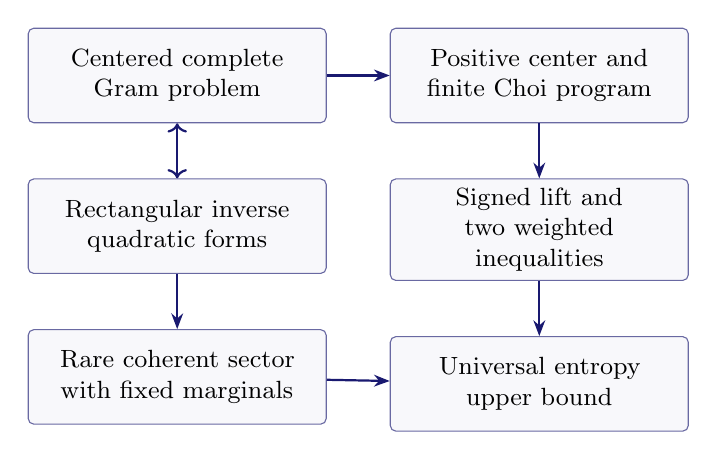
\begin{tikzpicture}[node distance=7mm and 8mm,
 box/.style={draw=MidnightBlue!65,rounded corners=2pt,align=center,
 fill=MidnightBlue!3,text width=3.55cm,minimum height=12mm,font=\small},
 arr/.style={-{Stealth[length=2mm]},thick,draw=MidnightBlue}]
\node[box] (gram) {Centered complete\\Gram problem};
\node[box,right=of gram] (choi) {Positive center and\\finite Choi program};
\node[box,below=of gram] (rect) {Rectangular inverse\\quadratic forms};
\node[box,below=of choi] (lift) {Signed lift and\\two weighted inequalities};
\node[box,below=of rect] (flag) {Rare coherent sector\\with fixed marginals};
\node[box,below=of lift] (entropy) {Universal entropy\\upper bound};
\draw[arr] (gram)--(choi);
\draw[arr,<->] (gram)--(rect);
\draw[arr] (choi)--(lift);
\draw[arr] (rect)--(flag);
\draw[arr] (lift)--(entropy);
\draw[arr] (flag)--(entropy);
\end{tikzpicture}
\caption{The upper inequality and the coherent converse meet at an exact
finite optimization.}
\label{fig:proof}
\end{figure}

The remainder follows this order. Sections~\ref{sec:gram}--\ref{sec:converse}
prove the main theorem. Section~\ref{sec:geometry} develops its geometry and
products. Sections~\ref{sec:petz}--\ref{sec:logarithmic} prove the divergence
extensions. Exact families, noise applications and the acquisition obstruction
occupy Sections~\ref{sec:examples}--\ref{sec:acquisition}.
\clearpage
% End sections/01-introduction

% Begin sections/02-definitions
\section{Coefficients and the exact Choi formula}
\label{sec:definitions}

All Hilbert spaces are finite dimensional. Write $\mathcal L(A)$ for the
operators on $A$ and $\States(A)$ for its density operators. Let
$\N:\mathcal L(A)\to\mathcal L(B)$ be completely positive and trace preserving
(CPTP), and put $d=\dim A$, $m=\dim B$. We use natural logarithms and the
Hilbert--Schmidt inner product $\ip{X}{Y}=\Tr X^*Y$. A superscript $*$ on a map
denotes its Hilbert--Schmidt adjoint. Reference extensions are denoted
$\N_R=\id_R\otimes\N$.

The Umegaki relative entropy is
\[
 D(\rho\|\sigma)=
 \begin{cases}
 \Tr\rho(\log\rho-\log\sigma),&\supp\rho\subseteq\supp\sigma,\\
 +\infty,&\text{otherwise}.
 \end{cases}
\]
Here $0\log0=0$, and logarithms on supports have their usual spectral meaning.
Unless explicitly stated otherwise, every ratio below has a strictly positive,
finite denominator. In a difference of divergences, each term must be finite;
an expression $\infty-\infty$ is never allowed. An empty supremum is zero.

\begin{definition}[Three reference-assisted coefficients]
\label{def:coefficients}
The complete and conditional-subtraction coefficients are
\begin{align}
 \etaC(\N)
 &=\sup_{\substack{R,\rho,\sigma\in\States(RA)\\
                   \rho_R=\sigma_R,\ 0<D(\rho\|\sigma)<\infty}}
       \frac{D(\N_R\rho\|\N_R\sigma)}{D(\rho\|\sigma)}, \label{eq:complete}\\
 \etaDel(\N)
 &=\sup_{\substack{R,\rho,\sigma\in\States(RA)\\
     D(\rho\|\sigma)<\infty,\ D(\rho\|\sigma)>D(\rho_R\|\sigma_R)}}
 \frac{D(\N_R\rho\|\N_R\sigma)-D(\rho_R\|\sigma_R)}
      {D(\rho\|\sigma)-D(\rho_R\|\sigma_R)}. \label{eq:conditional}
\end{align}
The conditional-mutual-information coefficient is
\begin{equation}
 \etaCM(\N)=
 \sup_{\substack{U,R,\rho\in\States(URA)\\ I(U;A|R)_\rho>0}}
 \frac{I(U;B|R)_{(\id_{UR}\otimes\N)(\rho)}}{I(U;A|R)_\rho}.
 \label{eq:conditional-mi}
\end{equation}
Both $U$ and $R$ may be quantum. Here
$I(U;A|R)=S(UR)+S(AR)-S(R)-S(URA)$ and $S(\rho)=-\Tr\rho\log\rho$.
\end{definition}

The coefficient in \eqref{eq:conditional-mi} has an additional conditioning
system. It differs from ordinary quantum mutual-information contraction,
\begin{equation}
 \etaMI(\N)=
 \sup_{\substack{R,\rho\in\States(RA)\\ I(R;A)_\rho>0}}
       \frac{I(R;B)_{\N_R(\rho)}}{I(R;A)_\rho}.
 \label{eq:ordinary-mi}
\end{equation}
The reference $R$ in \eqref{eq:ordinary-mi} is still arbitrary and quantum.
The adjective \emph{ordinary} does not mean that this reference is classical.

\begin{table}[htbp]
\centering\small
\begin{tabularx}{\textwidth}{@{}p{.19\textwidth}Y>{\raggedright\arraybackslash}p{.28\textwidth}@{}}
\toprule
Notation & Optimization & Reference requirement \\
\midrule
$\etaOrd$ & $D(\N\rho\|\N\sigma)/D(\rho\|\sigma)$ & No reference \\
$\etaMI$ & $I(R;B)/I(R;A)$ & One arbitrary quantum reference \\
$\etaP$ & $D(\N_R\rho\|\rho_R\otimes\N\sigma_A)/
 D(\rho\|\rho_R\otimes\sigma_A)$ & Second joint state is a product \\
$\etaC$ & \eqref{eq:complete} & Compared reference marginals equal \\
$\etaDel$ & \eqref{eq:conditional} & Reference divergence subtracted \\
$\etaCM$ & \eqref{eq:conditional-mi} & Separate message $U$ and memory $R$ \\
\bottomrule
\end{tabularx}
\caption{The optimizations are different. The product-reference coefficient
also optimizes $\sigma_A$; fixing it gives a further, generally different,
quantity.}
\label{tab:coefficients}
\end{table}

We use the \emph{unnormalized} Choi operator
\begin{equation}
 J_\N=\sum_{i,j=1}^d \ket{i}\bra{j}\otimes\N(\ket{i}\bra{j}),
 \qquad \Tr_B J_\N=I_A.
 \label{eq:choi}
\end{equation}
Write $J=J_\N$. Its Moore--Penrose inverse is $J^+$.

\begin{definition}[The Choi optimization]
\label{def:choi-optimization}
Let $M(\N)$ be the value of the finite SDP
\begin{equation}
\begin{aligned}
 \text{minimize}\quad &t\\
 \text{over}\quad &\sigma\in\States(B),\quad Z=Z^*\in\mathcal L(AB),
                  \quad t\in\mathbb R\\
 \text{subject to}\quad&
 \begin{pmatrix}J&I_A\otimes\sigma\\ I_A\otimes\sigma&Z\end{pmatrix}\succeq0,
 \qquad \Tr_B Z\preceq tI_A .
\end{aligned}
\label{eq:sdp}
\end{equation}
If it is infeasible, set $M(\N)=+\infty$. Set
$\beta(\N)=1/M(\N)$, with $1/\infty=0$.
The output density $\sigma$ in this program is an optimization center,
independent of the compared state pairs in \eqref{eq:complete}.
\end{definition}

\begin{theorem}[Exact reference-assisted Umegaki contraction]
\label{thm:main}
For every finite-dimensional CPTP map,
\begin{equation}
 \boxed{\quad \etaC(\N)=\etaDel(\N)=\etaCM(\N)=1-\beta(\N).\quad}
 \label{eq:main}
\end{equation}
Whenever \eqref{eq:sdp} is feasible its minimum is attained and $M\geq1$.
Equivalently,
\begin{equation}
 M=\min_{\substack{\sigma\in\States(B)\\
       \ran(I_A\otimes\sigma)\subseteq\ran J}}
 \norm{\Tr_B[(I_A\otimes\sigma)J^+(I_A\otimes\sigma)]}_\infty .
 \label{eq:inverse-choi}
\end{equation}
For every finite $R$ and state pair with $D(\rho\|\sigma)<\infty$,
\begin{equation}
 D(\N_R\rho\|\N_R\sigma)
 \leq (1-\beta)D(\rho\|\sigma)+\beta D(\rho_R\|\sigma_R).
 \label{eq:universal}
\end{equation}
The supremum in \eqref{eq:complete} can be approached with $\dim R\leq m^2+1$
and with both local marginals unchanged. In \eqref{eq:conditional-mi}, a
uniform classical bit $U$ suffices, with $\dim R\leq m^2+1$ and
$I(U;R)=I(U;A)=0$ exactly. If $d=1$, all three coefficients are zero.
\end{theorem}

The range condition in \eqref{eq:inverse-choi} is part of the formula. For
example, the identity channel on a space of dimension greater than one has
rank-one Choi operator and no feasible density $\sigma$. It therefore has
$M=\infty$ and coefficient one. Substituting a pseudoinverse while dropping the
range constraint would incorrectly make a finite expression determine this case.
Using a normalized Choi state would also change the scale of the optimization.

The definition-level distinction between conditional and ordinary mutual
information can now be summarized precisely.
\begin{proposition}[The coefficient hierarchy]
\label{prop:hierarchy}
With the quantities in \cref{tab:coefficients},
\begin{equation}
 0\leq\etaOrd(\N)\leq\etaMI(\N)=\etaP(\N)
 \leq\etaC(\N)=\etaDel(\N)=\etaCM(\N)\leq1.
 \label{eq:hierarchy}
\end{equation}
The identity $\etaMI=\etaP$ and the underlying information correspondences
are established in \cite[Corollary~3]{HGNW26}. A proof of the product-reference
identity is included in \cref{app:product-mi}; the complete/conditional
equalities are proved below.
\end{proposition}

Thus equality in \eqref{eq:main} does not identify ordinary MI with conditional
MI. For qubit depolarization at shrinkage $1/2$, the three successive values
$\etaOrd,\etaMI,\etaC$ are $1/4,1/3,3/8$; see \cref{thm:qubit-mi}.
Fixing both $A$ marginals to a faithful state also does not fix the second
joint state to a product. The former restriction leaves \eqref{eq:main}
unchanged, as proved in \cref{thm:prescribed}.
% End sections/02-definitions

% Begin sections/03-gram
\section{A finite Gram problem and its Choi solution}
\label{sec:gram}

The finite optimization enters before entropy. We first measure how far the
adjoint channel's output observables are from a common scalar center. Keeping
the whole Gram matrix is essential: its off-diagonal entries retain the tests
that arise from quantum references.

\subsection{Output supports and centered Gram matrices}

Let $B_{\mathrm s}=\supp\N(I_A)$. Every channel output is supported on
$B_{\mathrm s}$, since $X\succeq0$ implies $X\preceq cI_A$ for some $c$.
The same holds after every reference extension. If $C\succ0$ on $RA$, then
\[
 \N_R(C)\succeq c\,I_R\otimes\N(I_A)\succ0
 \quad\hbox{on }R\otimes B_{\mathrm s}
\]
for some $c>0$. We may therefore work on this fixed output space. A feasible
center in \eqref{eq:inverse-choi} must be supported there, so the optimization
is also unchanged by this reduction. Inverses of faithful output states below
are always taken on this actual output space. For notational ease call its
dimension $m$ in the proof; it is at most the original $m$.

Put $\Phi=\N^*$, a unital completely positive map. Choose a complex basis
$F_1,\ldots,F_n$ of $\mathcal L(B)$, where $n=m^2$, and define
\[
 \mathbf A=\begin{pmatrix}\Phi(F_1)\\ \vdots\\ \Phi(F_n)\end{pmatrix},
 \qquad \mathbf G=[\Phi(F_iF_j^*)]_{i,j=1}^n .
\]
Let $\eta_{\mathrm G}$ be the least $\eta\geq0$ for which some
$a\in\mathbb C^n$ obeys
\begin{equation}
 (\mathbf A-a\otimes I_A)(\mathbf A-a\otimes I_A)^*
 \preceq\eta\mathbf G .
 \label{eq:gram}
\end{equation}
Complete Schwarz gives feasibility at $\eta=1,a=0$. A bounded value of $\eta$
bounds $\norm{\mathbf A-a\otimes I}$ and hence $\norm a$, so a minimizing
center exists. A different finite tuple of output operators is a scalar
linear combination of this basis. Congruence of \eqref{eq:gram} therefore
controls every such tuple with the same linear centering functional.

\subsection{The rectangular dual problem}

For $C\succ0$ on $\mathbb C^k\otimes A$, a block column
$B:A\to\mathbb C^k\otimes A$ consists of $k$ matrices $B_i\in\mathcal L(A)$.
Define
\[
 q_C(B)=\Tr B^*C^{-1}B,\qquad
 \Tr_A B=(\Tr B_1,\ldots,\Tr B_k)^{\mathsf T}.
\]
Write $C'=\N_{\mathbb C^k}(C)$ and $B'=(\N(B_i))_i$.
The condition $\Tr_A B=0$ is blockwise; it is stronger than a single total
trace constraint.

\begin{lemma}[Complete Gram--rectangular identity]
\label{lem:rectangular}
Let
\begin{equation}
 \eta_{\mathrm{rect}}=
 \sup_{\substack{k,\ C\succ0,\ B\ne0\\ \Tr_A B=0}}
       \frac{q_{C'}(B')}{q_C(B)} .
 \label{eq:rectangular}
\end{equation}
Then $\eta_{\mathrm{rect}}=\eta_{\mathrm G}$.
The supremum is unchanged by requiring $\Tr C=1$ and $k\leq m^2$.
\end{lemma}

\begin{proof}
We give the weighted duality and the minimax step separately. For an output
block column $F=(F_i)_i$, Hilbert-space projection gives
\begin{equation}
 \sup_{\substack{B\ne0\\ \Tr_A B=0}}
 \frac{|\Tr B^*\Phi(F)|^2}{q_C(B)}
 =
 \inf_{a\in\mathbb C^k}
 \Tr C\,(\Phi(F)-a\otimes I)(\Phi(F)-a\otimes I)^* .
 \label{eq:weighted-duality}
\end{equation}
Indeed, on the block-column space the norm is
$\norm B_C^2=\Tr B^*C^{-1}B$. Its unrestricted dual norm at $T$ is
$\Tr CTT^*$. The Hilbert--Schmidt annihilator of the blockwise trace-zero
subspace is precisely $\{a\otimes I:a\in\mathbb C^k\}$. The norm of the
restricted functional is the distance to that annihilator in the dual norm,
which proves \eqref{eq:weighted-duality}. This argument works for complex
columns; no Hermiticity assumption on $B_i$ is made.

The unrestricted output dual norm at $F$ is
\[
 \Tr C'FF^*=\Tr C\,\Phi^{(k)}(FF^*).
\]
Dualizing the norm of $B\mapsto B'$ therefore expresses
\eqref{eq:rectangular}, for fixed $C$, as the supremum over nonzero $F$ of
the right side of \eqref{eq:weighted-duality} divided by this last quantity.
Apply \eqref{eq:gram} to the tuple $F$. Taking its expectation in $C$ proves
$\eta_{\mathrm{rect}}\leq\eta_{\mathrm G}$. Scaling $C$ to trace one
does not change either ratio.

Conversely, fix $0\leq e<\eta_{\mathrm G}$ and use the original basis tuple,
so $k=n$. For a density $C$ on $\mathbb C^n\otimes A$ set
\[
 f(C,a)=\Tr C\big[
    (\mathbf A-aI)(\mathbf A-aI)^*-e\mathbf G\big].
\]
This function is continuous and affine in $C$, and continuous and convex in
the real and imaginary parts of $a$. The density set is compact and convex;
the center space is convex. Sion's minimax theorem
\cite[Theorem~4.2]{Sion58} applies and gives
\begin{equation}
 \sup_C\inf_a f(C,a)
 =\inf_a\lambda_{\max}
    \big[(\mathbf A-aI)(\mathbf A-aI)^*-e\mathbf G\big]>0.
 \label{eq:gram-minimax}
\end{equation}
To justify the strict sign, the expression on the right is bounded below by
$(\norm a-\norm{\mathbf A})^2-e\norm{\mathbf G}$ when $\norm a$
is large. It is coercive and attains its minimum. A nonpositive minimum
would make \eqref{eq:gram} feasible at $e$, a contradiction.

Choose $C$ for which $\inf_a f(C,a)>0$. We can make it faithful.
The function $C\mapsto\inf_a f(C,a)$ is concave and is at least
$-e\norm{\mathbf G}$ on every density. Mixing $C$ with a sufficiently
small positive multiple of the maximally mixed density thus preserves the
strict sign. For the resulting faithful $C$, \eqref{eq:weighted-duality}
and norm duality supply a trace-zero block column whose ratio exceeds $e$.
Since $e$ can approach $\eta_{\mathrm G}$, the reverse inequality follows.
If $\eta_{\mathrm G}=0$ it is already immediate. This construction uses
$k=n=m^2$.
\end{proof}

\subsection{Stinespring centering}

Choose a minimal Stinespring isometry $V:A\to B\otimes E$ with
\[
 \Phi(Y)=V^*(Y\otimes I_E)V.
\]
In finite dimensions it can be obtained directly from a linearly independent
Kraus family, or from the positive Choi matrix. We use these standard
representations in the conventions of \cite{Stinespring55,Choi75}.

\begin{lemma}[Norm form of the centered Gram problem]
\label{lem:stinespring-center}
The Gram condition \eqref{eq:gram} at $e$ is equivalent to the existence of
$K:B\otimes E\to A$ and a complex-linear scalar functional $\alpha$ such that
\begin{equation}
 \norm K^2\leq e,\qquad
 K(Y\otimes I_E)V=\Phi(Y)-\alpha(Y)I_A
 \quad\text{for every }Y.
 \label{eq:stinespring-K}
\end{equation}
If there is a normalized map $S$ satisfying
\begin{equation}
 S(Y\otimes I_E)V=\alpha(Y)I_A,\qquad SV=I_A,
 \label{eq:normalized-center}
\end{equation}
then
\begin{equation}
 \eta_{\mathrm G}=1-\frac1{\inf_S\norm S^2}.
 \label{eq:gram-S}
\end{equation}
If no such normalized map exists, $\eta_{\mathrm G}=1$.
\end{lemma}

\begin{proof}
Let $T_i=(F_i^*\otimes I_E)V$ and let
$T:\bigoplus_{i=1}^n A\to B\otimes E$ be their row. Then
$T^*T=\mathbf G$. Put $Q=\mathbf A-aI$.
The inequality $QQ^*\preceq eT^*T$ says that
$K(Tv)=Q^*v$ is well defined and has norm at most $\sqrt e$.
Extend this map by zero on $(\ran T)^\perp$. Thus
$K(F_i^*\otimes I)V=\Phi(F_i^*)-\overline{a_i}I$.
The adjoint basis is a complex basis, so its values define $\alpha$ uniquely.
Conversely, \eqref{eq:stinespring-K} on that basis gives the Gram inequality
by taking the squared norm of every row combination. This proves the first
assertion without an implicit factorization theorem.

Put $L=V^*-K$. It obeys
$L(Y\otimes I)V=\alpha(Y)I$. If $t=\alpha(I)=0$, then $LV=0$ and
\[
 \norm{V^*-L}^2=\norm{I+LL^*}=1+\norm L^2\geq1.
\]
If $t\ne0$, write $L=tS$, so that $SV=I$, and decompose
$S=V^*+S_\perp$, where $S_\perp V=0$. Orthogonality gives
\begin{align}
 \norm{V^*-tS}^2
 &=|1-t|^2+|t|^2\norm{S_\perp}^2, \label{eq:t-minimization}\\
 \norm S^2&=1+\norm{S_\perp}^2. \label{eq:S-norm}
\end{align}
For fixed $r=\norm{S_\perp}^2$, the first expression has minimum
$r/(1+r)$ over complex $t$, attained at $t=1/(1+r)$.
Minimizing over normalized $S$ proves \eqref{eq:gram-S}. If none exists,
all feasible norms below one have been excluded, whereas $e=1$ was feasible.
\end{proof}

\subsection{The complex center is optimally positive}

\begin{lemma}[Inverse Choi and polar reduction]
\label{lem:polar}
The infimum over normalized centers in \eqref{eq:gram-S} equals the
minimum in \eqref{eq:inverse-choi}. In particular,
\[
 \eta_{\mathrm G}=1-\frac1{M(\N)}.
\]
\end{lemma}

\begin{proof}
Write
$V=\sum_j K_j\otimes\ket j$ and
$S=\sum_j L_j^*\otimes\bra j$, with the $K_j$ linearly independent.
Use the vectorization
$\ket{K}\!\rangle=\sum_i\ket i\otimes K\ket i$ and let $M_K,M_L$
have these vectors as columns. Expanding the matrix entries of
\eqref{eq:normalized-center} shows that, for a possibly complex $H$,
\begin{equation}
 M_LM_K^*=I_A\otimes H,\qquad \Tr H=1.
 \label{eq:kraus-center}
\end{equation}
More explicitly, the coefficient of $Y_{\mu\nu}$ in
$\sum_j L_j^*YK_j$ is
$\sum_j\overline{(L_j)_{\mu a}}(K_j)_{\nu b}$.
Equation \eqref{eq:kraus-center} is precisely the statement that this is
$\delta_{ab}\overline{H_{\mu\nu}}$.
Thus the associated functional is $\alpha(Y)=\Tr(H^*Y)$.

Since $J=M_KM_K^*$ and $M_K$ has independent columns,
\eqref{eq:kraus-center} has a solution exactly when
\begin{equation}
 \ran(I_A\otimes H^*)\subseteq\ran J,
 \label{eq:complex-range}
\end{equation}
and that solution is
$M_L=(I_A\otimes H)J^+M_K$. Consequently
\begin{equation}
 \norm S^2=
 \norm{\Tr_B[(I\otimes H)J^+(I\otimes H^*)]}_\infty .
 \label{eq:complex-objective}
\end{equation}
The remaining $A$ matrix equals $(SS^*)^{\mathsf T}$ under this
vectorization, which explains why its operator norm is the stated one.

Partial-trace cyclicity in the $B$ factor rewrites the matrix inside the
norm as $\Tr_B[J^+(I\otimes H^*H)]$. Also,
$\ran H^*=\ran|H|$. Let $a=\Tr|H|\geq|\Tr H|=1$.
Replacing $H$ by the density $\sigma=|H|/a$ preserves
\eqref{eq:complex-range} and divides the positive matrix in
\eqref{eq:complex-objective} by $a^2$.
This is the required positivity argument; restricting a complex center to a
Hermitian one without it would not suffice.

Conversely, every admissible density $\sigma$ supplies a normalized center
by \eqref{eq:kraus-center}. The admissible densities form a closed subset
of the compact density set, and their objective is continuous, because $J$
is fixed. If this subset is nonempty, its minimum is attained. Since
$SV=I$, $\norm S\geq1$, proving $M\geq1$.

Finally, for a positive $J$ and Hermitian $A_0$, the generalized Schur
complement gives
\begin{equation}
 \begin{pmatrix}J&A_0\\ A_0&Z\end{pmatrix}\succeq0
 \quad\Longleftrightarrow\quad
 \ran A_0\subseteq\ran J,\quad Z\succeq A_0J^+A_0.
 \label{eq:schur}
\end{equation}
To verify it, test the block form on vectors in $\ker J$ to obtain the
range condition. On $\supp J$, complete the square in the first block;
the residual form is $Z-A_0J^+A_0$. This proves both directions,
including singular $J$. Apply \eqref{eq:schur} to $A_0=I_A\otimes\sigma$.
The partial trace is positive, and equality is attained by
$Z=A_0J^+A_0$, so the inverse formulation and \eqref{eq:sdp} agree.
\end{proof}

Combining \cref{lem:rectangular,lem:stinespring-center,lem:polar} yields the
finite identity that will be used in both directions of the entropy theorem:
\begin{equation}
 \eta_{\mathrm{rect}}=\eta_{\mathrm G}=1-\beta(\N).
 \label{eq:quadratic-optimum}
\end{equation}
% End sections/03-gram

% Begin sections/04-upper
\section{A signed lift and the universal upper bound}
\label{sec:upper}

This section applies the signed-observable method to a particular comparison
channel: erasure. The distinction between observable reconstruction and a
physical channel is crucial. The constructed map is linear and adjoint
preserving, but need not preserve positive observables.

\subsection{Both square inequalities}

Assume first $1<M<\infty$. Choose an optimal positive center $\sigma$ and
the normalized map $S$ from \cref{lem:polar}. Set
\[
 Q=S-V^*,\qquad QV=0,\qquad
 r=\norm Q^2=M-1,\qquad \alpha(Y)=\Tr\sigma Y.
\]
The defining equation for $S$ gives
\[
 \Phi(Y)-\alpha(Y)I
 =-Q(I-VV^*)(Y\otimes I_E)V.
\]
Taking its square and using $Q^*Q\preceq rI$ proves
\begin{align}
 (\Phi(Y)-\alpha(Y)I)^*(\Phi(Y)-\alpha(Y)I)
 &\preceq r\,[\Phi(Y^*Y)-\Phi(Y)^*\Phi(Y)], \label{eq:square-right}\\
 (\Phi(Y)-\alpha(Y)I)(\Phi(Y)-\alpha(Y)I)^*
 &\preceq r\,[\Phi(YY^*)-\Phi(Y)\Phi(Y)^*]. \label{eq:square-left}
\end{align}
The second follows by applying the first to $Y^*$; positivity of $\sigma$
makes $\alpha$ adjoint preserving. Tensoring $Q,V$ with $I_R$ proves both
inequalities for every finite reference and every operator on $RB$.
The amplified center is $(\id_R\otimes\alpha)(Y)\otimes I_A$; it need
not commute with the other reference operators.

Put $e=r/(1+r)=1-\beta$ and define the erasure channel, with retention
probability $e$, by
\[
 \E_e(X)=eX\oplus(1-e)\Tr X.
\]
The erasure output algebra is $\mathcal L(A)\oplus\mathbb C$.
Define the observable map $\mathcal J:\mathcal L(B)\to
\mathcal L(A)\oplus\mathbb C$ by
\begin{equation}
 (\mathcal JY)_{\mathrm r}
 =\frac{\Phi(Y)-(1-e)\alpha(Y)I}{e},
 \qquad
 (\mathcal JY)_{\mathrm e}=\alpha(Y).
 \label{eq:signed-lift}
\end{equation}
Then $\E_e^*\mathcal J=\Phi$, equivalently $\mathcal J^*\E_e=\N$.
Direct expansion, valid also for noncommuting amplified centers, gives
\begin{align}
 &\Phi(Y^*Y)-\E_e^*((\mathcal JY)^*(\mathcal JY)) \notag\\
 &\quad=
 \Phi(Y^*Y)-\Phi(Y)^*\Phi(Y)
 -\frac{1-e}{e}(\Phi(Y)-\alpha(Y)I)^*
                         (\Phi(Y)-\alpha(Y)I)\succeq0 .
 \label{eq:lift-defect}
\end{align}
There is a second identity with $YY^*$ and the opposite square order.
The final sign in \eqref{eq:lift-defect} is exactly
\eqref{eq:square-right}, since $(1-e)/e=1/r$.

For a positive matrix $\omega$, write
$L_\omega(X)=\omega X$ and $R_\omega(X)=X\omega$.
Taking expectations of the two amplified identities in an arbitrary faithful
state $\omega_{RA}$ yields the separate weighted inequalities
\begin{equation}
 \mathcal J_R^* L_{\E_{e,R}(\omega)}\mathcal J_R
       \preceq L_{\N_R(\omega)},\qquad
 \mathcal J_R^* R_{\E_{e,R}(\omega)}\mathcal J_R
       \preceq R_{\N_R(\omega)} .
 \label{eq:two-weights}
\end{equation}
The $YY^*$ identity gives the left weight and the $Y^*Y$ identity gives
the right weight. Each holds for every $\omega$ with the \emph{same} map
$\mathcal J_R=\id_R\otimes\mathcal J$. This state independence will also
allow different states in the two weights in \cref{sec:petz}.

\subsection{Inverse quadratic duality and the entropy metric}

For completeness, we prove the exact comparison mechanism rather than treating
the signed map as a simulator. This is the mechanism of
\cite[Lemma~S6 and Theorem~S5]{ZW26v3}, in the erasure specialization.

\begin{lemma}[Inverse quadratic comparison]
\label{lem:inverse-duality}
Let $A,B$ be positive definite operators on finite Hilbert spaces and
$T$ a linear map with $T^*AT\preceq B$. Then
\[
 \ip{T^*z}{B^{-1}T^*z}\leq\ip z{A^{-1}z}.
\]
\end{lemma}
\begin{proof}
Completing the square gives
\[
 \ip z{A^{-1}z}
 =\sup_x\{2\Rea\ip xz-\ip x{Ax}\}.
\]
Restrict this supremum to $x=Ty$ and use
$\ip{Ty}{ATy}\leq\ip y{By}$. The resulting supremum over $y$
equals $\ip{T^*z}{B^{-1}T^*z}$ by the same identity.
\end{proof}

For $\omega\succ0$ and Hermitian $H$, define
\begin{equation}
 g_\omega(H)=
 \int_0^1
 \ip H{[(1-u)L_\omega+uR_\omega]^{-1}H}\dd u .
 \label{eq:bkm}
\end{equation}
In an eigenbasis of $\omega$, with eigenvalues $\lambda_i>0$,
\begin{equation}
 g_\omega(H)=\sum_{i,j}|H_{ij}|^2
 \frac{\log\lambda_i-\log\lambda_j}{\lambda_i-\lambda_j},
 \label{eq:bkm-spectral}
\end{equation}
where the divided difference is $1/\lambda_i$ on the diagonal.
Indeed, integrating $[(1-u)\lambda_i+u\lambda_j]^{-1}$ proves this formula.
It is the Hessian of $F(\omega)=\Tr\omega\log\omega$, as follows by
differentiating the spectral logarithm. For example, the derivative formula
\[
 D\log_\omega(H)=
 \int_0^\infty(\omega+sI)^{-1}H(\omega+sI)^{-1}\dd s
\]
has exactly the divided differences in \eqref{eq:bkm-spectral}. Thus
$g_\omega$ is the Bogoliubov--Kubo--Mori (BKM) metric.

Add the inequalities \eqref{eq:two-weights} with weights $1-u,u$ and apply
\cref{lem:inverse-duality} to $z=\E_{e,R}(H)$.
The reconstruction identity gives $\mathcal J_R^*z=\N_R(H)$.
Integrating in $u$ proves
\begin{equation}
 g_{\N_R(\omega)}(\N_R(H))
 \leq g_{\E_{e,R}(\omega)}(\E_{e,R}(H)).
 \label{eq:bkm-erasure}
\end{equation}
All inverses here act on the actual output supports; the two erasure
branches are faithful when $0<e<1$.

\begin{lemma}[Affine-path integration and finite-entropy boundaries]
\label{lem:entropy-integration}
For faithful states $\rho,\tau$, put $H=\rho-\tau$. Then
\begin{equation}
 D(\rho\|\tau)=\int_0^1(1-s)\,g_{\tau+sH}(H)\dd s.
 \label{eq:entropy-integral}
\end{equation}
If $D(\rho\|\tau)<\infty$ and $\zeta$ is faithful, the common mixtures
$\rho_\epsilon=(1-\epsilon)\rho+\epsilon\zeta$ and
$\tau_\epsilon=(1-\epsilon)\tau+\epsilon\zeta$ satisfy
$D(\rho_\epsilon\|\tau_\epsilon)\to D(\rho\|\tau)$.
The same convergence holds after any CPTP map, on its actual output support.
\end{lemma}
\begin{proof}
Relative entropy is the Bregman remainder of $F$ on the trace-one affine
space. Its first derivative remainder vanishes, and Taylor's integral
formula gives \eqref{eq:entropy-integral}.

For the boundary assertion, finite relative entropy implies
$\rho\preceq c\tau$ for some finite $c$. Hence
$\rho_\epsilon\preceq\max(c,1)\tau_\epsilon$.
The term $\Tr\rho_\epsilon\log\rho_\epsilon$ converges because
$x\log x$ is continuous at zero. Diagonalize $\tau_\epsilon$.
For any eigenvalue $\lambda_i(\epsilon)\to0$, its diagonal weight
$w_i(\epsilon)$ in $\rho_\epsilon$ is at most
$\max(c,1)\lambda_i(\epsilon)$, so
$w_i(\epsilon)|\log\lambda_i(\epsilon)|\to0$.
On the spectral subspace of eigenvalues bounded away from zero,
continuous functional calculus gives convergence to $\Tr\rho\log\tau$.
There are finitely many eigenvalues, so the cross term converges as well.
A channel preserves $\rho\preceq c\tau$; its common mixture state is
faithful on the fixed output support. The same argument applies there.
\end{proof}

\subsection{The universal Umegaki inequality}

Integrate \eqref{eq:bkm-erasure} along the path in
\eqref{eq:entropy-integral}. The orthogonal erasure branches give
\[
 D(\E_{e,R}\rho\|\E_{e,R}\tau)
 =eD(\rho\|\tau)+(1-e)D(\rho_R\|\tau_R).
\]
This proves \eqref{eq:universal} for faithful states.
\Cref{lem:entropy-integration} extends it to every finite-input-entropy pair;
the reference terms converge by the same lemma.

If $M=1$, \eqref{eq:square-right} has $r=0$, so
$\Phi(Y)=\alpha(Y)I$ for every $Y$. This is a replacer channel
$\N(X)=\Tr(X)\sigma$, and \eqref{eq:universal} is equality with $e=0$.
If $M=\infty$, use the identity comparison channel instead of erasure and
take $\mathcal J=\Phi$. Stinespring Schwarz gives both weighted
inequalities \eqref{eq:two-weights}. The preceding metric and path
argument proves ordinary data processing, which is \eqref{eq:universal}
with $e=1$. No assertion about a finite inverse-Choi center is needed in
this case.

Subtracting $D(\rho_R\|\tau_R)$ now gives
$\etaDel\leq1-\beta$, and equal-reference pairs give
$\etaC\leq1-\beta$.
For any $\rho_{URA}$, apply \eqref{eq:universal} with reference $UR$ to
the pair
\[
 \rho_{URA},\qquad \rho_U\otimes\rho_{RA}.
\]
Its input relative entropy is $I(U;RA)$ and its reference relative entropy
is $I(U;R)$. Their difference is $I(U;A|R)$, and the output difference
is $I(U;B|R)$. Both terms are finite in finite dimensions because the
first state is supported in the product of its marginals' supports.
This proves $\etaCM\leq1-\beta$ for arbitrary quantum $U,R$, under the
explicit definition \eqref{eq:conditional-mi}.
% End sections/04-upper

% Begin sections/05-converse
\section{The coherent converse with exactly fixed marginals}
\label{sec:converse}

The rectangular problem in \cref{lem:rectangular} is not itself an entropy
ratio. Its conversion into one is the main converse construction. A new
reference direction makes a rectangular matrix into an off-diagonal
Hermitian perturbation. Making that direction rare selects the inverse
quadratic weight needed for the exact optimum.

\begin{lemma}[A positive coherent family]
\label{lem:coherent-family}
Let $C\succ0$ be a trace-one state on $R_0A$, let
$B:A\to R_0A$ be nonzero with $\Tr_A B=0$, and let $\tau\succ0$ be a
state on $A$. Put $R=R_0\oplus\mathbb C r$, $q=1-p$, and
\begin{equation}
 \omega_p=\begin{pmatrix}qC&0\\0&p\tau\end{pmatrix},\qquad
 H_p=\begin{pmatrix}0&\sqrt{pq}\,B\\
                    \sqrt{pq}\,B^*&0\end{pmatrix},
 \qquad \rho_{p,h}=\omega_p+hH_p .
 \label{eq:coherent-family}
\end{equation}
For $0<p<1$, these are faithful states whenever $|h|$ is sufficiently
small in an interval independent of $p$. Both their $R$ and $A$
marginals equal those of $\omega_p$ exactly.
\end{lemma}
\begin{proof}
The Schur complement of $qC$ in $\rho_{p,h}$ is
\[
 p\big(\tau-h^2B^*C^{-1}B\big).
\]
It is positive definite, for example, when
$h^2\norm{\tau^{-1/2}B^*C^{-1}B\tau^{-1/2}}<1$.
This condition is independent of $p$. The perturbation has total trace
zero. Its reference marginal is zero because each block of $B$ has trace
zero. Its input marginal is zero because it is off diagonal in the
reference direct sum. Thus $\Tr_AH_p=\Tr_RH_p=0$.
\end{proof}

\begin{lemma}[The inverse weight selected by a rare sector]
\label{lem:rare-bkm}
For the family \eqref{eq:coherent-family},
\begin{equation}
 \lim_{p\downarrow0}\frac{g_{\omega_p}(H_p)}
                              {2p\log(1/p)}=q_C(B).
 \label{eq:rare-bkm}
\end{equation}
The corresponding output limit is $q_{C'}(B')$, where
$C'=\N_{R_0}(C)$ and $B'=\N(B)$ blockwise.
\end{lemma}
\begin{proof}
Let $c_i>0$ and $v_j>0$ be eigenvalues of $C$ and $\tau$, and write
$B_{ij}$ in these eigenbases. Only the cross-sector entries contribute to
\eqref{eq:bkm-spectral}; both orientations contribute equally. Hence
\begin{equation}
 g_{\omega_p}(H_p)=
 2pq\sum_{i,j}|B_{ij}|^2
 \frac{\log(qc_i)-\log(pv_j)}{qc_i-pv_j}.
 \label{eq:coherent-bkm-exact}
\end{equation}
Coincident arguments are interpreted by continuity. For each fixed
$(i,j)$, division by $2p\log(1/p)$ makes its factor converge to
$|B_{ij}|^2/c_i$. There are finitely many terms, and their sum is
$\Tr B^*C^{-1}B$.
The output has the same block form, with faithful $C'$ and
$\tau'=\N(\tau)$ on the fixed output support. The identical
divided-difference computation proves the second limit.
\end{proof}

\begin{proof}[Completion of \cref{thm:main}]
For each fixed $p$, analyticity at the faithful state $\omega_p$ gives
\[
 D(\omega_p+hH_p\|\omega_p)
       =\frac{h^2}{2}g_{\omega_p}(H_p)+O_p(h^3).
\]
The same expansion applies to the output. The denominator's quadratic
coefficient is strictly positive. Thus \cref{lem:rare-bkm} gives
\begin{equation}
 \lim_{p\downarrow0}\lim_{h\to0}
 \frac{D(\N_R(\omega_p+hH_p)\|\N_R\omega_p)}
      {D(\omega_p+hH_p\|\omega_p)}
       =\frac{q_{C'}(B')}{q_C(B)}.
 \label{eq:ordered-entropy-limit}
\end{equation}
Every pair on the left has exactly the same reference marginal.
Taking the supremum over $C,B$ and using
\eqref{eq:quadratic-optimum} proves
$\etaC\geq1-\beta$.

For clarity, the limit statement produces ordinary finite admissible
pairs: given a desired accuracy, first choose $C,B$ with nearly optimal
rectangular ratio, then choose a sufficiently small $p$, and finally a
sufficiently small nonzero $h$. No uniform bound on the $O_p(h^3)$
remainder as $p\downarrow0$ is claimed or required.

To obtain a conditional-MI witness, let a uniform classical bit $U$
select $\omega_p+hH_p$ and $\omega_p-hH_p$. Its average is
exactly $\omega_p$. By \cref{lem:coherent-family},
$I(U;R)=I(U;A)=0$ exactly. Also,
\begin{align*}
 I(U;RA)
 &=\tfrac12D(\omega_p+hH_p\|\omega_p)
   +\tfrac12D(\omega_p-hH_p\|\omega_p),\\
 I(U;RB)
 &=\tfrac12D(\N_R(\omega_p+hH_p)\|\N_R\omega_p)
   +\tfrac12D(\N_R(\omega_p-hH_p)\|\N_R\omega_p).
\end{align*}
Subtracting $I(U;R)=0$ makes these the two conditional mutual
informations. Their ordered local limits give the same rectangular
ratio. Thus $\etaCM\geq1-\beta$.
Equal-reference pairs are admissible in the conditional coefficient, so
$\etaDel\geq\etaC$. The upper bounds already proved give all equalities.

\Cref{lem:rectangular} supplies $\dim R_0\leq m^2$; only the one
additional direction was used. The stated reference bounds follow.
When $d=1$, every channel is a replacer and every admissible coefficient
is zero. For a nontrivial replacer with $d>1$, admissible finite pairs
exist but their output numerator is zero; the same conclusion holds.
\end{proof}

\begin{remark}[Information in correlations and its size]
The binary label in the construction is invisible in each subsystem
separately, although it is visible in their correlations. This explains why
classical-reference intuition need not give the coefficient. It does not
ensure a large absolute signal. For fixed $p$, the information vanishes
quadratically as $h\to0$, and its quadratic scale is itself
$p\log(1/p)$ as the sector becomes rare.
\end{remark}
% End sections/05-converse

% Begin sections/06-geometry
\section{Support, harmonic duality and exact products}
\label{sec:geometry}

The inverse-Choi formula has consequences that are easier to see in matrix
geometry than in entropy ratios. We develop them explicitly, retaining the
positive CP-replacer coefficient as a distinct, previously established object.

\subsection{Complete output rows and strict contraction}

Let $P$ be the support projection of $J$ and define
\begin{equation}
 E_J=\ker\Tr_A(I_{AB}-P).
 \label{eq:complete-row-space}
\end{equation}
This is an output subspace, not an environment or an erasure flag.
For $b\in B$,
\[
 \ip b{\Tr_A(I-P)b}
 =\sum_{i=1}^d\norm{(I-P)(\ket i\otimes b)}^2.
\]
Consequently $E_J$ is the largest subspace with
$A\otimes E_J\subseteq\ran J$.
A density $\sigma$ is feasible in \eqref{eq:inverse-choi} exactly when
its range lies in $E_J$.

\begin{corollary}[Strict-contraction criterion]
\label{cor:strict}
For every channel, the following are equivalent:
\[
 \etaC(\N)<1,\qquad
 E_J\ne\{0\},\qquad
 J\succeq a I_A\otimes\sigma
 \ \text{for some }\sigma\in\States(B),\ a>0 .
\]
The same criterion holds for $\etaDel$ and $\etaCM$.
\end{corollary}
\begin{proof}
The first two conditions are equivalent by the nonempty feasible set in
\eqref{eq:inverse-choi}. The last implies the range inclusion and hence
the second. Conversely, take a unit vector $b\in E_J$ and let $a>0$
be at most the smallest positive eigenvalue of $J$. Then
$J\succeq aP\succeq aI_A\otimes\ket b\bra b$.
\end{proof}

In channel language the last condition is positive CP-replacer minorization.
With the notation of \cite[Definition~7, equation~(3.25)]{GHNW26}, put
\begin{equation}
 \alpha_+(\N)=\max\{\Tr H:H\succeq0,\ I_A\otimes H\preceq J\}.
 \label{eq:positive-doeblin}
\end{equation}
If $\alpha_+>0$, writing $H=\alpha_+\sigma$ gives
$\N=\alpha_+\mathcal R_\sigma+(1-\alpha_+)\mathcal Q$ with $\mathcal Q$
CPTP, except that at $\alpha_+=1$ the channel is itself a replacer.
Here $\mathcal R_\sigma(X)=\Tr(X)\sigma$.
Positivity of $H$ is required. The Doeblin optimization over arbitrary
Hermitian $H$ in \cite{GHNW26} is a different coefficient.

\subsection{The harmonic dual}

Assume $E_J\ne0$. Compress $J^+$ to the positive definite operator
$K$ on $A\otimes E_J$. The compression is positive definite because
$A\otimes E_J\subseteq\ran J$; invariance of this subspace under $J$
is not required.

\begin{theorem}[Matrix harmonic dual]
\label{thm:harmonic}
With $H_\theta=\Tr_A[(\theta\otimes I_{E_J})K]$,
\begin{equation}
 \boxed{\quad
 \beta(\N)=\min_{\theta\in\States(A)}\Tr H_\theta^{-1}.
 \quad}
 \label{eq:harmonic-dual}
\end{equation}
Every $H_\theta$ is positive definite, including for singular $\theta$.
\end{theorem}
\begin{proof}
The inverse-Choi objective can be written
\[
 M=\min_{\sigma\in\States(E_J)}\max_{\theta\in\States(A)}
       \Tr K(\theta\otimes\sigma^2).
\]
The function is affine in $\theta$ and convex in $\sigma$:
for fixed $\theta$ it is $\Tr H_\theta\sigma^2$, a positive quadratic
form. Both density sets are compact and convex, so convex minimax applies.
If $K\succeq cI$, then $H_\theta\succeq cI$ because $\Tr\theta=1$.
Here partial-trace cyclicity identifies $H_\theta$ with the positive
matrix
$\Tr_A[(\theta^{1/2}\otimes I)K(\theta^{1/2}\otimes I)]$.
Weighted Hilbert--Schmidt Cauchy--Schwarz gives
\[
 1=(\Tr\sigma)^2
 \leq(\Tr H_\theta^{-1})(\Tr H_\theta\sigma^2).
\]
Equality holds at
$\sigma=H_\theta^{-1}/\Tr H_\theta^{-1}$.
Thus
\[
 M=\max_\theta\frac1{\Tr H_\theta^{-1}}
   =\frac1{\min_\theta\Tr H_\theta^{-1}},
\]
which proves the formula.
\end{proof}

\begin{theorem}[Exact tensor products]
\label{thm:products}
For arbitrary finite channels,
\begin{align}
 \beta(\N_1\otimes\N_2)&=\beta(\N_1)\beta(\N_2), \label{eq:beta-product}\\
 \eta(\N_1\otimes\N_2)
 &=1-(1-\eta(\N_1))(1-\eta(\N_2)), \label{eq:eta-product}
\end{align}
where $\eta$ is any coefficient in \eqref{eq:main}.
\end{theorem}
\begin{proof}
First the feasible support spaces multiply, including zero spaces.
Let $P_i=\supp J_i$, $S_i=\Tr_{A_i}P_i$ and $d_i=\dim A_i$.
Since $0\preceq P_i\preceq I$, $0\preceq S_i\preceq d_iI$.
The space $E_{J_i}$ is the eigenspace of $S_i$ at $d_i$.
After the natural tensor-factor reordering,
the product support projection is $P_1\otimes P_2$ and its output
partial trace is $S_1\otimes S_2$.
An eigenvalue product equals $d_1d_2$ exactly when each factor equals
$d_i$. Hence
\[
 E_{J_1\otimes J_2}=E_{J_1}\otimes E_{J_2}.
\]
If a factor is zero, the product $\beta$ is zero and
\eqref{eq:beta-product} follows.

Otherwise, product choices of $\sigma$ in the primal give
$M_{12}\leq M_1M_2$, since their inverse forms and positive
partial-trace matrices tensor. Therefore
$\beta_{12}\geq\beta_1\beta_2$.
On the product support the compressed inverse is $K_1\otimes K_2$.
Choose minimizing $\theta_1,\theta_2$ in \eqref{eq:harmonic-dual}.
Their product produces $H_{\theta_1}\otimes H_{\theta_2}$, so the dual
gives
$\beta_{12}\leq(\Tr H_{\theta_1}^{-1})(\Tr H_{\theta_2}^{-1})
=\beta_1\beta_2$.
The entropy identity follows from \cref{thm:main}.
\end{proof}

This is an all-pairs, variable-reference product law. It does not assert
tensorization of an ordinary coefficient or a fixed-equilibrium entropy-decay
constant; the latter belong to a different setting~\cite{GR22}.

\subsection{A sharp comparison with positive replacer weight}

\begin{theorem}[Harmonic bounds and sharp Doeblin comparison]
\label{thm:doeblin-comparison}
If $E_J\ne0$, set
\[
 K_E=\left.P_{E_J}(\Tr_AJ^+)P_{E_J}\right|_{E_J},
 \qquad h(J)=\Tr_{E_J}K_E^{-1}.
\]
If $E_J=0$, put $h(J)=0$. Then
\begin{equation}
 h(J)\leq\beta(\N)\leq d\,h(J),\qquad
 \boxed{\ \alpha_+(\N)\leq\beta(\N)\leq d^2\alpha_+(\N).\ }
 \label{eq:doeblin-comparison}
\end{equation}
The factor $d^2$ cannot be decreased uniformly in channels of input
dimension $d\geq2$.
\end{theorem}
\begin{proof}
The zero-space case follows from \cref{cor:strict}.
For feasible $\sigma$ write
$T_\sigma=\Tr_B[(I\otimes\sigma)J^+(I\otimes\sigma)]$.
It is positive and
$\Tr T_\sigma=\Tr K_E\sigma^2$.
Its norm lies between its trace divided by $d$ and its trace.
The minimum possible trace is $1/h(J)$, attained at
$\sigma=K_E^{-1}/\Tr K_E^{-1}$ by Cauchy--Schwarz.
Thus $1/(dh)\leq M\leq1/h$, which proves the first bounds.

If $J\succeq aI\otimes\sigma$, $a>0$, then
\[
 \begin{pmatrix}J&I\otimes\sigma\\
 I\otimes\sigma&(I\otimes\sigma)/a\end{pmatrix}\succeq0.
\]
Indeed, subtract $\diag(J-aI\otimes\sigma,0)$; the remaining matrix
is $I\otimes\sigma$ tensored with the positive scalar matrix
$\left(\begin{smallmatrix}a&1\\1&1/a\end{smallmatrix}\right)$.
This is feasible in \eqref{eq:sdp} with $t=1/a$, proving
$\alpha_+\leq\beta$.

For a positive operator $T$ on $AB$ one has
\begin{equation}
 T\preceq dI_A\otimes\Tr_AT.
 \label{eq:partialtrace-domination}
\end{equation}
For a rank-one term $\ket v\bra v$, conjugation by the inverse square
root of its $B$ marginal on that marginal's support makes the vector's
squared norm its Schmidt rank, at most $d$. This proves
\eqref{eq:partialtrace-domination} for that term. Sum rank-one terms
to obtain the stated inequality.

When $J\succ0$, apply \eqref{eq:partialtrace-domination} to $J^{-1}$
and invert. It gives
$J\succeq d^{-1}I_A\otimes(\Tr_AJ^{-1})^{-1}$, so
$\alpha_+\geq h/d$. For singular $J$, let
$J_\epsilon=J+\epsilon I$. Then
\[
 \Tr_AJ_\epsilon^{-1}
 =\epsilon^{-1}\Tr_A(I-P)+\Tr_AJ^++O(\epsilon).
\]
Decompose $B=E_J\oplus E_J^\perp$. The leading matrix is zero on the
first block and positive definite on the second. The block inverse,
or its Schur complement, consequently converges to
$P_{E_J}K_E^{-1}P_{E_J}$: its $E_J$ block converges to $K_E^{-1}$,
and the other blocks vanish. Taking the limit in the preceding feasible
matrix inequality again gives $\alpha_+\geq h/d$.
Combine this with $\beta\leq dh$ to prove
$\beta\leq d^2\alpha_+$.

For sharpness, use any orthogonal unitary error basis with probabilities
$p_g>0$. The calculation in \cref{thm:error-basis} gives
$\beta=d^4/\sum_g p_g^{-1}$. Also,
$\alpha_+=d^2\min_g p_g$: testing $I\otimes H\preceq J$ against
each maximally entangled error-basis vector gives
$\Tr H/d\leq dp_g$, and scalar $H$ attains the minimum bound.
Let one probability tend to zero while the others stay bounded away
from zero. Then $\beta/\alpha_+\to d^2$.
\end{proof}

The qualitative minorization criterion and its information-theoretic
applications are prior work~\cite{GHNW26,HGNW26}. The comparison
\eqref{eq:doeblin-comparison} quantifies how the exact coefficient can improve
that baseline. Its factor is dimension dependent; for $n$ qubits it is $4^n$.

\subsection{Prescribed input marginals}

\begin{theorem}[Faithful marginal padding and support dependence]
\label{thm:prescribed}
Let $\omega_A$ be faithful. The value of $\etaC(\N)$ is unchanged
if both compared input marginals are required to equal $\omega_A$.
Reference dimension at most $m^2+2$ suffices to approach it.
The binary witnesses for $\etaCM$ may also have
$\rho_A=\omega_A$ and $I(U;A)=I(U;R)=0$ exactly.

For nonfaithful $\omega_A$, either fixing both input marginals to
$\omega_A$, or fixing only the second input marginal in
\eqref{eq:complete}, gives the coefficient of the restricted channel
$\N|_{\mathcal L(\supp\omega_A)}$.
Thus these values depend on $\omega_A$ only through its support.
\end{theorem}
\begin{proof}
The witnesses in \cref{sec:converse} already have a common input marginal,
say $\nu_A$. Choose $0<a<1$ so small that
$\tau_A=(\omega_A-a\nu_A)/(1-a)\succeq0$.
Append one orthogonal reference flag and put
\[
 \widetilde\rho=a\rho\oplus(1-a)\tau_A,\qquad
 \widetilde\sigma=a\sigma\oplus(1-a)\tau_A.
\]
The reference marginals agree, and both input marginals are exactly
$\omega_A$. Orthogonal direct sums give
$D(\widetilde\rho\|\widetilde\sigma)=aD(\rho\|\sigma)$
before and after the channel, so the ratio is unchanged.
The same padding, with the same weights in both bit branches, preserves
the two independence identities and scales both Holevo informations by
$a$. This uses one additional reference direction.

If $S=\supp\omega_A$, positivity forces every joint state with that
input marginal to be supported in $R\otimes S$. If only the second
input marginal is fixed, finite $D(\rho\|\sigma)$ forces the first
joint state into that support as well. The upper bound is therefore
the restricted channel's coefficient. On $S$, $\omega_A$ is faithful,
so the preceding padding construction gives the matching lower bound.
A one-dimensional support gives zero.
\end{proof}

The comparison state in this theorem can be correlated with its reference.
It is not fixed to $\rho_R\otimes\omega_A$.
There is consequently no conflict with the distinct product-reference
coefficient in \cref{tab:coefficients}, or with entropy contraction toward a
specified equilibrium.
In particular, fixing only the second input marginal is the
input-dependent complete coefficient of \cite[Definition~12]{GHNW26};
for faithful $\omega_A$ it too has the common value in \eqref{eq:main}.
% End sections/06-geometry

% Begin sections/07-petz
\section{Universality for regular modular Petz divergences}
\label{sec:petz}

The entropy upper bound used a single baseline state in its two weighted
inequalities. Their state independence permits a stronger use: the left
weight can come from one state and the right weight from another. This
controls resolvent divergences directly, without first integrating an
entropy Hessian.

\subsection{The divergence and its exact generator class}

\begin{definition}[Regular modular Petz generators]
\label{def:regular-f}
Let $f:(0,\infty)\to\mathbb R$ be nonaffine and operator convex, with
\[
 f(1)=f'(1)=0,\qquad f(0+)<\infty,\qquad
 \ell_f=\lim_{x\to\infty}\frac{f(x)}x<\infty.
\]
Its modular Petz divergence on faithful states is
\begin{equation}
 D_f(\rho\|\sigma)=
 \ip{\sigma^{1/2}}{f(L_\rho R_\sigma^{-1})\sigma^{1/2}}.
 \label{eq:modular-petz}
\end{equation}
For positive semidefinite states use its continuous spectral extension:
if $\rho=\sum_i r_i\ket{u_i}\bra{u_i}$ and
$\sigma=\sum_j s_j\ket{v_j}\bra{v_j}$, then
\[
 D_f(\rho\|\sigma)=
 \sum_{i,j}F_f(r_i,s_j)|\ip{u_i}{v_j}|^2,
 \qquad F_f(a,b)=b f(a/b)\quad(a,b>0),
\]
with $F_f(0,b)=bf(0+)$, $F_f(a,0)=a\ell_f$ and $F_f(0,0)=0$.
\end{definition}

This is the modular, or standard Petz, divergence~\cite{Petz86}. It is not the maximal
quantum $f$-divergence and not the hockey-stick integral construction
of \cite{HT24}. In particular, an equality for another divergence with the
same classical restriction would not imply the theorem below.

For any divergence $V$ used here, define $\eta_V^{\mathrm c}$ and
$\eta_V^\Delta$ by replacing $D$ in \eqref{eq:complete} and
\eqref{eq:conditional}. Define, explicitly,
\begin{equation}
 \mathcal I_V(U;A|R)_\rho=
 V(\rho_{URA}\|\rho_U\otimes\rho_{RA})
 -V(\rho_{UR}\|\rho_U\otimes\rho_R),
 \label{eq:generalized-information}
\end{equation}
and let $\eta_{\mathcal I_V}$ be the output-to-input ratio of this
quantity, with a strictly positive finite input and finite terms.
All auxiliary systems are arbitrary finite quantum systems.
For $V=D$ this is ordinary conditional mutual information. For other
$V$ it denotes exactly the displayed difference, without an optimization
over comparison states.

\begin{theorem}[Exact regular modular Petz coefficients]
\label{thm:petz}
For every generator in \cref{def:regular-f} and every finite channel,
\begin{equation}
 \eta_{D_f}^{\mathrm c}(\N)
 =\eta_{D_f}^{\Delta}(\N)
 =\eta_{\mathcal I_{D_f}}(\N)
 =1-\beta(\N).
 \label{eq:petz-coefficients}
\end{equation}
For arbitrary state pairs and references,
\begin{equation}
 D_f(\N_R\rho\|\N_R\sigma)
 \leq(1-\beta)D_f(\rho\|\sigma)
       +\beta D_f(\rho_R\|\sigma_R).
 \label{eq:petz-upper}
\end{equation}
The sharpness bounds $\dim R\leq m^2+1$ and a binary classical
auxiliary independent of both local marginals remain valid.
\end{theorem}

\subsection{Positive resolvents and endpoint integrability}

\begin{lemma}[The precise integral representation]
\label{lem:resolvent-representation}
For $f$ in \cref{def:regular-f} there is a positive measure $\nu$ on
$(0,\infty)$ such that
\begin{equation}
 f(x)=\int_{(0,\infty)}\frac{(x-1)^2}{x+s}\dd\nu(s),
 \qquad
 \int_{(0,\infty)}(1+s^{-1})\dd\nu(s)
 =f(0+)+\ell_f=:k_f\in(0,\infty).
 \label{eq:resolvent-representation}
\end{equation}
\end{lemma}
\begin{proof}
Franz--Hiai's representation \cite[Theorem~2.2]{FH14}, at the base
point one, is
\[
 f(x)=\gamma(x-1)^2+
       \int_{[0,\infty)}
       \frac{(x-1)^2}{(x+s)(1+s)^2}\dd\mu(s),
 \qquad \gamma\geq0,\quad
 \int(1+s)^{-3}\dd\mu(s)<\infty.
\]
The affine part is zero by normalization. Finite recession slope
forces $\gamma=0$; finite $f(0+)$ excludes an atom at zero.
Set $\dd\nu(s)=(1+s)^{-2}\dd\mu(s)$.
As $x\downarrow0$, the nonnegative integrands increase to $1/s$.
As $x\uparrow\infty$, their ratios to $x$ increase to one for $x\geq1$.
Monotone convergence gives
$f(0+)=\int s^{-1}\dd\nu$ and $\ell_f=\int\dd\nu$.
Nonaffineness means the measure is nonzero, proving strict positivity.
\end{proof}

Let $f_s(x)=(x-1)^2/(x+s)$. Commutation of left and right multiplication
in the modular calculus gives
\begin{equation}
 D_{f_s}(\rho\|\sigma)
 =Q_s(\rho,\sigma):=
 \ip{\rho-\sigma}{(L_\rho+sR_\sigma)^{-1}(\rho-\sigma)}
 \quad(s>0).
 \label{eq:resolvent-divergence}
\end{equation}
To check it, move $\Delta-I$, with $\Delta=L_\rho R_\sigma^{-1}$,
onto $\sigma^{1/2}$ in \eqref{eq:modular-petz}; its value is
$(\rho-\sigma)\sigma^{-1/2}$. The factors of $R_\sigma^{1/2}$
cancel in $(\Delta+sI)^{-1}
=R_\sigma(L_\rho+sR_\sigma)^{-1}$, giving
\eqref{eq:resolvent-divergence}. Thus
$D_f=\int Q_s\dd\nu(s)$ for faithful states.

\subsection{Two-state weights give the upper inequality}

Write $e=1-\beta$ and initially suppose $0<e<1$.
In \eqref{eq:two-weights}, use $\rho$ for the left-weight state
and $\sigma$ for the right-weight state. Adding with weight $s>0$
gives
\[
 \mathcal J_R^*
 (L_{\E_{e,R}(\rho)}+sR_{\E_{e,R}(\sigma)})\mathcal J_R
 \preceq L_{\N_R(\rho)}+sR_{\N_R(\sigma)}.
\]
Apply \cref{lem:inverse-duality} with
$z=\E_{e,R}(\rho-\sigma)$ and use reconstruction. This proves
\[
 Q_s(\N_R\rho,\N_R\sigma)
 \leq Q_s(\E_{e,R}\rho,\E_{e,R}\sigma).
\]
The two erasure branches are orthogonal, and $Q_s$ is homogeneous of
degree one in the pair. Consequently the right side is
$eQ_s(\rho,\sigma)+(1-e)Q_s(\rho_R,\sigma_R)$.
Positive integration proves \eqref{eq:petz-upper}.
For $e=1$ take the identity comparison and $\mathcal J=\Phi$, as in
\cref{sec:upper}; for $e=0$ the replacer gives equality with the
reference divergence.

These statements extend continuously to all PSD state pairs.
For the scalar perspective of $f_s$,
\begin{equation}
 0\leq\frac{(a-b)^2}{a+sb}\leq a+\frac bs
 \quad(a,b\geq0),
 \label{eq:perspective-bound}
\end{equation}
with $0/0=0$. It is continuous, including at $(0,0)$.
Spectral calculus for the commuting operators $L_\rho,R_\sigma$
therefore gives continuity of $Q_s$. Equivalently one can approximate
this continuous scalar function uniformly by polynomials on the
compact spectral square. Its spectral expression and
\eqref{eq:perspective-bound} bound $Q_s$ by $1+s^{-1}$.
\Cref{lem:resolvent-representation} supplies an integrable bound, so
dominated convergence proves continuity of $D_f$ and the boundary
passage in \eqref{eq:petz-upper}.

Subtracting the reference term proves the two relative-divergence upper
bounds. Applying the same inequality with reference $UR$ to
$(\rho_{URA},\rho_U\otimes\rho_{RA})$ proves the upper bound for
\eqref{eq:generalized-information}. The reference subtraction is
legitimate even when $U$ is quantum.

\subsection{The matching local and coherent converse}

\begin{lemma}[Regular Petz coherent Hessians]
\label{lem:petz-hessian}
For \eqref{eq:coherent-family} at each fixed $p$,
\[
 D_f(\omega_p+hH_p\|\omega_p)
       =\frac{h^2}{2}g^f_{\omega_p}(H_p)+o_p(h^2),
\]
and
\begin{equation}
 \lim_{p\downarrow0}\frac{g^f_{\omega_p}(H_p)}{2p}
        =k_fq_C(B).
 \label{eq:petz-rare-limit}
\end{equation}
The output limit is $k_fq_{C'}(B')$.
\end{lemma}
\begin{proof}
For one resolvent, \eqref{eq:resolvent-divergence} gives exactly
\[
 Q_s(\omega+hH,\omega)
 =h^2\ip H{(L_{\omega+hH}+sR_\omega)^{-1}H}.
\]
At fixed faithful $\omega$, choose $h$ so that
$\omega+hH\succeq\omega/2$. The right quadratic form is then
at most twice its value with $\omega+hH$ replaced by $\omega$.
This bounds the second-order quotient by an integrable function of $s$.
Taking $h\to0$ under the positive integral is therefore justified.
For the coherent block family, diagonalization as in
\cref{lem:rare-bkm} gives
\begin{equation}
 g^{f_s}_{\omega_p}(H_p)
 =2pq\sum_{i,j}|B_{ij}|^2
   \left(\frac1{qc_i+spv_j}+
         \frac1{pv_j+sqc_i}\right).
 \label{eq:petz-hessian-exact}
\end{equation}
After division by $2p$, its summand is bounded above by
$(1+s^{-1})|B_{ij}|^2/c_i$ and converges to that same quantity
as $p\downarrow0$. There are finitely many $(i,j)$.
Dominated convergence against $\nu$ proves
\eqref{eq:petz-rare-limit}. Faithfulness of $C',\tau'$ on the actual
output support gives the identical proof at the output.
\end{proof}

\begin{proof}[Completion of \cref{thm:petz}]
Take $h\to0$ at each fixed $p$, and then $p\downarrow0$.
The common positive factor $k_f$ in
\eqref{eq:petz-rare-limit} cancels, leaving
$q_{C'}(B')/q_C(B)$. The same-reference lower bound is therefore
$\eta_{\mathrm{rect}}=1-\beta$.

For the binary auxiliary of \cref{sec:converse}, the compared joint
states are the two equally weighted blocks and their common average.
The direct-sum formula for $D_f$ makes
$\mathcal I_{D_f}(U;A|R)$ the average of the two local divergences;
the reference term vanishes exactly. Both signs have the same
second-order coefficient in \cref{lem:petz-hessian}. This gives the
matching information lower bound. The conditional coefficient contains
the equal-reference pairs. Together with the upper bounds already
proved, this establishes \eqref{eq:petz-coefficients} with the stated
reference dimensions. Empty one-dimensional cases have value zero.
\end{proof}

Umegaki entropy is not a member of \cref{def:regular-f}: the normalized
generator $x\log x-x+1$ has infinite recession slope. Its independent
proof in Sections~\ref{sec:upper}--\ref{sec:converse} is therefore
necessary.
% End sections/07-petz

% Begin sections/08-logarithmic
\section{Petz R\'enyi and quantum Chernoff contraction}
\label{sec:logarithmic}

Taking a logarithm is not innocuous for contraction coefficients. We show the
required scalar inequality and then prove sharpness locally. For Chernoff
divergence, an additional compact-order Taylor estimate justifies the
optimization over the order.

For $0<\alpha<1$, define
\[
 Q_\alpha(\rho,\sigma)=\Tr\rho^\alpha\sigma^{1-\alpha},\qquad
 D_\alpha(\rho\|\sigma)=-\frac1{1-\alpha}\log Q_\alpha(\rho,\sigma).
\]
Define quantum Chernoff divergence by
\[
 C_Q(\rho,\sigma)=-\log\inf_{0<\alpha<1}Q_\alpha(\rho,\sigma).
\]
If the logarithm's argument is zero the value is $+\infty$.
The complete and reference-subtracted coefficients, and the generalized
information coefficient, use precisely
\eqref{eq:generalized-information} and the finiteness conventions in
\cref{sec:definitions}. In particular, $\mathcal I_{D_\alpha}$ is not an
optimized or sandwiched R\'enyi conditional mutual information.

\begin{theorem}[Logarithmic extensions]
\label{thm:renyi-chernoff}
For every fixed $0<\alpha<1$ and every finite channel,
\begin{align}
 \eta_{D_\alpha}^{\mathrm c}(\N)
 =\eta_{D_\alpha}^{\Delta}(\N)
 =\eta_{\mathcal I_{D_\alpha}}(\N)&=1-\beta(\N), \label{eq:renyi-exact}\\
 \eta_{C_Q}^{\mathrm c}(\N)
 =\eta_{C_Q}^{\Delta}(\N)
 =\eta_{\mathcal I_{C_Q}}(\N)&=1-\beta(\N). \label{eq:chernoff-exact}
\end{align}
Both divergences $V$ satisfy, on their finite-input-divergence domains,
\begin{equation}
 V(\N_R\rho\|\N_R\sigma)
 \leq(1-\beta)V(\rho\|\sigma)+\beta V(\rho_R\|\sigma_R).
 \label{eq:log-upper}
\end{equation}
A reference of dimension at most $m^2+1$ and a binary classical
auxiliary independent of each local marginal suffice for sharpness.
\end{theorem}

\subsection{The logarithmic upper bound}

For fixed $\alpha$, the normalized generator
\[
 f_\alpha(x)=\frac{1-\alpha+\alpha x-x^\alpha}{1-\alpha}
\]
belongs to \cref{def:regular-f}. Operator convexity follows from
operator concavity of $x^\alpha$; also
$f_\alpha(0+)=1$ and $\ell_{f_\alpha}=\alpha/(1-\alpha)$.
Its modular divergence is
$D_{f_\alpha}=(1-Q_\alpha)/(1-\alpha)$.
For clarity, the operator concavity of the power follows from the
convergent integral
\[
 x^\alpha=\frac{\sin(\pi\alpha)}{\pi}
       \int_0^\infty \frac{x}{x+s}s^{\alpha-1}\dd s .
\]
Each matrix function $X(X+sI)^{-1}=I-s(X+sI)^{-1}$ is operator
concave: operator convexity of the inverse follows by applying the
inverse-quadratic variational identity to each vector.
Thus \eqref{eq:petz-upper}, with $e=1-\beta$, gives
\begin{equation}
 Q_{\alpha,\mathrm{out}}\geq
       eQ_{\alpha,\mathrm{in}}+(1-e)Q_{\alpha,R}.
 \label{eq:hellinger-affine}
\end{equation}
For positive $a,b$, weighted arithmetic--geometric mean gives
$ea+(1-e)b\geq a^e b^{1-e}$.
Taking minus logarithms in \eqref{eq:hellinger-affine} therefore proves
\eqref{eq:log-upper} for $D_\alpha$.
More explicitly, with
$x=D_{\alpha,\mathrm{in}}-D_{\alpha,R}\geq0$,
\[
 D_{\alpha,\mathrm{out}}-D_{\alpha,R}
 \leq-\frac{\log(1-e+e e^{-(1-\alpha)x})}{1-\alpha}
 \leq ex.
\]
This is the logarithmic step needed for the conditional ratio.

Multiplying by $1-\alpha$ gives the same affine bound for
$-\log Q_\alpha$. Taking the supremum over $0<\alpha<1$ yields
\[
 C_{Q,\mathrm{out}}
 \leq eC_{Q,\mathrm{in}}+(1-e)C_{Q,R},
\]
since the supremum of the sum is at most the sum of the suprema.
This proves the Chernoff upper bound. Subtraction and the product
comparison in \eqref{eq:generalized-information} give all the upper
coefficient bounds.

\subsection{Boundary passage without an endpoint-uniform assumption}

For fixed interior $\alpha$, matrix powers are continuous on PSD matrices,
so \eqref{eq:hellinger-affine} extends directly to arbitrary states.
The same inequality also proves data processing when $e=1$.
In particular a finite input divergence has finite reference and output
divergences.

For the Chernoff boundary, mix a pair with a common faithful state $\tau$.
Each $Q_\alpha$ is jointly concave. One way to see precisely the needed
fact is to use \eqref{eq:resolvent-divergence}: its variational inverse
formula makes $Q_s$ jointly convex in the state pair. Positive
integration gives joint convexity of $D_{f_\alpha}$, hence joint
concavity of $Q_\alpha$. Boundary continuity for fixed $\alpha$ extends
that conclusion to PSD states. Therefore
\[
 Q_\alpha(\rho_\epsilon,\sigma_\epsilon)
 \geq(1-\epsilon)Q_\alpha(\rho,\sigma)+\epsilon.
\]
Taking the infimum gives the corresponding lower bound on
$\inf_\alpha Q_\alpha(\rho_\epsilon,\sigma_\epsilon)$.
For every fixed interior order, continuity gives the reverse
limsup bound; then take the infimum over that fixed order.
Consequently
\begin{equation}
 \inf_\alpha Q_\alpha(\rho_\epsilon,\sigma_\epsilon)
 \longrightarrow \inf_\alpha Q_\alpha(\rho,\sigma).
 \label{eq:chernoff-boundary}
\end{equation}
On the finite-Chernoff domain the limit is positive, so its negative
logarithm converges. This argument does not assert uniform continuity
of matrix powers in $\alpha$ at singular endpoints.

\subsection{Local R\'enyi sharpness}

At every faithful coincident pair,
$-\log Q_\alpha=(1-Q_\alpha)+O((1-Q_\alpha)^2)$.
Thus $D_\alpha$ and $D_{f_\alpha}$ have the same nonzero
second-order coefficient under a traceless perturbation.
Apply \cref{lem:petz-hessian} at fixed $p$, then send $p$ to zero:
the regular-generator factor cancels between input and output.
This gives the lower bound in \eqref{eq:renyi-exact}.
For the uniform bit, $Q_\alpha$ is the average of its two block
values. Its logarithm has the same second-order expansion, and the
reference term is zero. This proves sharpness of the generalized
information coefficient as well.

\subsection{The optimized Chernoff converse}

\begin{lemma}[Uniform local order optimization]
\label{lem:chernoff-local}
For \eqref{eq:coherent-family}, fix $0<p<1$. Uniformly for
$0\leq\alpha\leq1$,
\begin{equation}
 Q_\alpha(\omega_p+hH_p,\omega_p)
   =1-h^2 A_{\alpha,p}+O_p(|h|^3),
 \qquad
 A_{\alpha,p}=pq\sum_{i,j}|B_{ij}|^2
 K_\alpha(qc_i,pv_j),
 \label{eq:chernoff-taylor}
\end{equation}
where
\[
 K_\alpha(a,b)=
 \frac{(a^\alpha-b^\alpha)(a^{1-\alpha}-b^{1-\alpha})}
      {(a-b)^2},
 \qquad K_\alpha(a,a)=\frac{\alpha(1-\alpha)}a.
\]
The maximum of $A_{\alpha,p}$ is attained at $\alpha=1/2$, and
\begin{equation}
 C_Q(\omega_p+hH_p,\omega_p)
 =h^2A_{1/2,p}+O_p(|h|^3),\qquad
 \lim_{p\downarrow0}\frac{A_{1/2,p}}p=q_C(B).
 \label{eq:chernoff-rare}
\end{equation}
\end{lemma}
\begin{proof}
We first compute the coefficient. For a diagonal baseline with eigenvalues
$a,b$ and an off-diagonal entry $h z$, the second-order change of
$\Tr(\omega+hH)^\alpha\omega^{1-\alpha}$ is
$-|z|^2K_\alpha(a,b)h^2$. This follows, for example, by the
second divided difference of $x^\alpha$: its contribution at the $a$
entry is
\[
 a^{1-\alpha}\frac{b^\alpha-a^\alpha-\alpha a^{\alpha-1}(b-a)}
                         {(b-a)^2}|z|^2,
\]
and the analogous contribution at $b$ has the opposite first-order
linear term. Adding them gives $-K_\alpha(a,b)|z|^2$.
The coincident-eigenvalue formula is its continuous limit.
Summing the cross-sector entries
$z=\sqrt{pq}\,B_{ij}$ proves \eqref{eq:chernoff-taylor}.

The remainder is genuinely uniform at this fixed $p$.
Choose $h_0>0$ so that $\omega_p+hH_p$ is bounded below by a positive
multiple of the identity for $|h|\leq h_0$. On this compact faithful
set the map
$(h,\alpha)\mapsto \exp(\alpha\log(\omega_p+hH_p))$
has continuous third derivatives in $h$ for $\alpha\in[0,1]$.
They are bounded on the compact parameter rectangle. Taylor's theorem
therefore gives one $O_p(|h|^3)$ bound for all those orders.

For $a\ne b$, the numerator in $K_\alpha$ is
\[
 a+b-a^\alpha b^{1-\alpha}-a^{1-\alpha}b^\alpha
 \leq a+b-2\sqrt{ab}.
\]
Equality holds at $\alpha=1/2$ by arithmetic--geometric mean.
The coincident case uses $\alpha(1-\alpha)\leq1/4$.
Hence every nonnegative summand is maximized at one half, and
$K_{1/2}(a,b)=(\sqrt a+\sqrt b)^{-2}$.
The uniform remainder now permits taking the infimum in
\eqref{eq:chernoff-taylor} before the local limit in $h$.
Taking a logarithm gives the first assertion in \eqref{eq:chernoff-rare}.
Finally,
\[
 \frac{A_{1/2,p}}p
 =q\sum_{i,j}\frac{|B_{ij}|^2}
                   {(\sqrt{qc_i}+\sqrt{pv_j})^2}
 \longrightarrow\sum_{i,j}\frac{|B_{ij}|^2}{c_i}.
\]
This is a finite sum; its terms are bounded by $|B_{ij}|^2/c_i$.
\end{proof}

\begin{proof}[Completion of \cref{thm:renyi-chernoff}]
The same Chernoff lemma applies at the output, so its ordered local and
rare-sector ratio is $q_{C'}(B')/q_C(B)$.
For the binary auxiliary, the two compared direct-sum blocks have equal
weights. Their $Q_\alpha$ is the average of the values at $h$ and $-h$,
uniformly in $\alpha$; the coefficient in
\eqref{eq:chernoff-taylor} is unchanged.
The reference divergence vanishes exactly. Hence the same local
Chernoff ratio proves the generalized information lower bound.
The conditional ratio again contains the complete one.
Use \eqref{eq:quadratic-optimum} and the already proved upper bounds.
The construction has the same reference size as before.
\end{proof}

\begin{corollary}[Faithful marginal constraints for the extensions]
\label{cor:extended-padding}
The complete coefficients in \cref{thm:petz,thm:renyi-chernoff}
are unchanged when both input marginals are prescribed to a faithful
state $\omega_A$. The binary generalized-information witnesses may
also have input marginal $\omega_A$ and be independent of each local
subsystem. Reference dimension at most $m^2+2$ suffices.
\end{corollary}
\begin{proof}
Use the padding in \cref{thm:prescribed}, with one fixed
$0<a<\lambda_{\min}(\omega_A)$; since every input marginal is at
most $I_A$, the residual density is positive.
For modular $D_f$, both local divergences scale exactly by $a$.
For $D_\alpha$, the padded value is
\[
 -\frac1{1-\alpha}
 \log\!\left[1-a+a\exp(-(1-\alpha)D_\alpha)\right]
 =aD_\alpha+O(D_\alpha^2)
\]
at a coincident pair. For Chernoff it is
$-\log(1-a+a e^{-C_Q})=aC_Q+O(C_Q^2)$, since an increasing
affine map commutes with the infimum of $Q_\alpha$.
Consequently the local $h\to0$ ratios in the sharpness construction
are unchanged. The same block calculation applies to the uniform-bit
comparison, whose reference term is exactly zero. Only one reference
direction is added.
\end{proof}

This corollary concerns faithful prescribed marginals.
For the nonfaithful, second-marginal-only restriction, the Umegaki
support argument in \cref{thm:prescribed} must not be transferred to
these divergences. For example, take the identity channel,
$\sigma=\ket0\bra0$ and
$\rho=\diag(1-t,t)$, $0<t<1$. The regular modular, interior-order
Petz R\'enyi and Chernoff divergences of this pair are positive and
finite, so the restricted ratio is one, whereas restricting the
channel itself to $\supp\sigma$ gives a one-dimensional input and
coefficient zero.

The uniformity used in \cref{lem:chernoff-local} is only at a fixed
faithful $\omega_p$. No Taylor remainder uniform in the rare-sector weight
or in singular states has been used.
In fact, an endpoint extension at Petz order zero is false.

\begin{proposition}[A zero-order obstruction]
\label{prop:zero-order}
For qubit depolarization with shrinkage $1/2$, all three coefficients
defined from
$D_0(\rho\|\sigma)=-\log\Tr(P_\rho\sigma)$ are zero.
For every fixed $0<\alpha<1$, the three corresponding $D_\alpha$
coefficients equal $3/8$.
\end{proposition}
\begin{proof}
For any reference,
$\N_R(\rho)=\rho/2+\rho_R\otimes I_2/4$ has support
$\supp\rho_R\otimes\mathbb C^2$. Therefore
$D_0(\N_R\rho\|\N_R\sigma)=D_0(\rho_R\|\sigma_R)$.
Every conditional numerator is zero; equal-reference numerators also
vanish. The same support identity with reference $UR$ proves the
generalized-information assertion. Positive finite input denominators
exist, for example from a pure input versus $I_2/2$, or a uniform bit
encoded in two orthogonal inputs. The interior value follows from
\cref{thm:renyi-chernoff,thm:depolarizing}.
\end{proof}

Thus fixed-order exactness is not a uniform extremizer statement as the order
approaches zero. Orders above one, sandwiched R\'enyi divergences, maximal
divergences and hockey-stick divergences are not included. An explicit
higher-order counterexample is recorded in \cref{app:order-ten}.
% End sections/08-logarithmic

% Begin sections/09-examples
\section{Exact families and the mutual-information separation}
\label{sec:examples}

We now evaluate the formula and compare the optimizations in
\cref{tab:coefficients}. Throughout this section, $\eta(\N)$ denotes the
common value in \eqref{eq:main}, or any of the complete, conditional-difference
and generalized-information coefficients proved equal to it in
\cref{thm:petz,thm:renyi-chernoff}. It never denotes ordinary MI or
ordinary unreferenced relative-entropy contraction.

\subsection{Replacers and identity channels}

For a replacer $\mathcal R_\tau(X)=\Tr(X)\tau$, $J=I_A\otimes\tau$.
The feasible density $\sigma=\tau$ gives inverse objective one:
\[
 \Tr_B[(I\otimes\tau)J^+(I\otimes\tau)]
 =\Tr(\tau\tau^+\tau)\,I_A=I_A.
\]
Since $M\geq1$, $M=1$, $\beta=1$ and $\eta=0$, including pure
replacers. If $d>1$, an identity or isometric channel has no complete
output row in its rank-one Choi support, so $\beta=0$ and $\eta=1$.
These examples also show why singularity alone does not determine
whether contraction is strict.

\subsection{Every finite classical channel}

Let $W(y|x)$ be a stochastic matrix and regard it as the quantum channel
that first measures $x$ and then prepares the output basis state $y$.
Define the common positive-output set
$Y_0=\{y:W(y|x)>0\text{ for all }x\}$.

\begin{theorem}[The classical harmonic formula with quantum references]
\label{thm:classical}
For every finite stochastic matrix,
\begin{equation}
 \boxed{\quad
 \eta(W)=1-\min_{\theta\in\Delta_X}
 \sum_{y\in Y_0}
       \left(\sum_x\frac{\theta_x}{W(y|x)}\right)^{-1}.
 \quad}
 \label{eq:classical-harmonic}
\end{equation}
An empty sum is zero. The bound is sharp even when the channel input
register is required to be classical; the untouched reference can be
quantum.
\end{theorem}
\begin{proof}
The Choi operator is diagonal with entries $W(y|x)$.
Its feasible centers are supported on the span of $Y_0$.
For a possibly nondiagonal density $\sigma$ on that span, the
$x$th diagonal entry of its inverse form is
\[
 \sum_{y\in Y_0}\frac{(\sigma^2)_{yy}}{W(y|x)}
 \geq\sum_{y\in Y_0}\frac{\sigma_{yy}^2}{W(y|x)}.
\]
The remaining input matrix is diagonal. Removing off-diagonal center
entries cannot increase its norm, so
\begin{equation}
 M(W)=\min_{\substack{s_y\geq0\\\sum_{y\in Y_0}s_y=1}}
          \max_x\sum_{y\in Y_0}\frac{s_y^2}{W(y|x)}.
 \label{eq:classical-primal}
\end{equation}
If $Y_0$ is empty the program is infeasible. Otherwise, convex minimax
and scalar weighted Cauchy--Schwarz give
\[
 M=\max_{\theta\in\Delta_X}
 \left[\sum_{y\in Y_0}
       \left(\sum_x\frac{\theta_x}{W(y|x)}\right)^{-1}\right]^{-1}.
\]
Taking the reciprocal proves \eqref{eq:classical-harmonic}.

To justify sharpness with a classical input, reconsider the minimax
proof of \cref{lem:rectangular}. Both $\mathbf A$ and $\mathbf G$ are
block diagonal in $x$. Dephasing $C$ in that input basis preserves
every minimax objective, and it preserves faithfulness.
For the weighted projection in \eqref{eq:weighted-duality}, the
Riesz representative has the form $C(\Phi(F)-aI)$ at its minimizing
center; it is also block diagonal in $x$ and its blockwise trace is
zero by the center's first-order optimality condition.
Thus the witnessing $B$ can be chosen block diagonal in $x$.
Choose $\tau$ diagonal in that basis in \eqref{eq:coherent-family}.
The coherent states are then classical on the channel input, while
their off-diagonal entries occur in the reference. The converse
arguments for all the stated divergences retain this property.
\end{proof}

For the $k$-symbol symmetric channel, with diagonal $a>0$, off-diagonal
$b>0$ and $a+(k-1)b=1$, permutation symmetry and convexity in
\eqref{eq:classical-primal} make $s_y=1/k$ optimal. Hence
\begin{equation}
 \eta(W)=1-\frac{k^2}{1/a+(k-1)/b}.
 \label{eq:symmetric-reference}
\end{equation}
This differs from its ordinary classical KL coefficient
\begin{equation}
 \eta_{\mathrm{KL,class}}(W)=\frac{(a-b)^2}{a+b},
 \label{eq:symmetric-classical}
\end{equation}
whose full elementary proof is in \cref{app:classical}.
The general binary-input reduction for ordinary classical SDPI is
established in \cite[Theorem~1]{OP21}; the classical formula is not
claimed as a new method here.

\begin{table}[htbp]
\centering
\begin{tabular}{@{}llll@{}}
\toprule
Channel & Parameters & Ordinary classical KL & Quantum-reference $\eta$\\
\midrule
Symmetric ternary & $a=3/5,\ b=1/5$ & $1/5$ & $8/35$\\
Symmetric ternary & $a=9/10,\ b=1/20$ & $289/380$ & $289/370$\\
$k$-symbol exclusion & $a=0,\ b=1/(k-1)$ & $1/(k-1)$ & $1$\\
\bottomrule
\end{tabular}
\caption{A classical channel can retain substantially more distinguishability
in correlations with a quantum reference. The ordinary column restricts the
input pair itself to probability distributions.}
\label{tab:classical}
\end{table}

The ternary triple $(.9,.05,.05)$ and its permutations is discussed in
\cite[Section~9.4]{Balsu26} for multihypothesis Chernoff quantities.
Those testing exponents are different from both columns in
\cref{tab:classical}. Neither the symmetric channel nor established
classical testing formulas are being relabelled as a new construction.
The reference-assisted value follows from \eqref{eq:classical-harmonic}.

For the exclusion channel on $k\geq3$ symbols, every output has a zero
transition, so $Y_0$ is empty and $\eta=1$; its ordinary KL coefficient
is $1/(k-1)$. The separation also persists without zero entries.
Choose $a=k^{-3}$ and $b=(1-a)/(k-1)$. Then
\[
 \eta(W)>1-\frac1k,\qquad
 \eta_{\mathrm{KL,class}}(W)<b<\frac1{k-1}.
\]
The first inequality follows from $1/a=k^3$ in
\eqref{eq:symmetric-reference}; the second follows from $0<a<b$ in
\eqref{eq:symmetric-classical}. The ratio of the two coefficients is
therefore unbounded as the alphabet grows.

\subsection{Depolarizing channels in all dimensions}

For $d\geq2$ let
\[
 \D_\lambda(X)=\lambda X+(1-\lambda)\Tr(X)\frac{I_d}{d},
 \qquad -\frac1{d^2-1}\leq\lambda\leq1.
\]
This is its full CP interval.

\begin{theorem}[Exact complete depolarizing coefficient]
\label{thm:depolarizing}
On the full CP interval,
\begin{equation}
 \boxed{\qquad
 \eta(\D_\lambda)=
 \frac{(d^2-1)\lambda^2}{1+(d^2-2)\lambda}.
 \qquad}
 \label{eq:depolarizing}
\end{equation}
In dimension one the channel is a replacer and its coefficient is zero.
\end{theorem}
\begin{proof}
In the interior of the interval,
$J=\lambda\ket\Omega\bra\Omega+(1-\lambda)I_{d^2}/d$
is positive definite, where $\ket\Omega=\sum_i\ket{ii}$.
Its eigenvalues are
\[
 a=\frac{1+(d^2-1)\lambda}{d}\quad\text{once},\qquad
 b=\frac{1-\lambda}{d}\quad\text{$d^2-1$ times}.
\]
It is invariant under $\overline U\otimes U$.
Conjugating a feasible center by $U$ leaves the inverse objective
unchanged. That objective is convex: the difference between the
weighted average of the two quadratic matrices and the matrix of the
averaged center is a positive partial trace of a square.
Averaging over the $d^2$ Weyl conjugations therefore makes $I_d/d$
optimal. The inverse Choi marginal is scalar, giving
\[
 M=\frac{\Tr J^{-1}}{d^3}
 =\frac1{d^2}
 \left(\frac1{1+(d^2-1)\lambda}+\frac{d^2-1}{1-\lambda}\right)
 =\frac{1+(d^2-2)\lambda}
        {(1-\lambda)(1+(d^2-1)\lambda)} .
\]
Substitution into $1-1/M$ proves \eqref{eq:depolarizing}.

At the negative CP endpoint the kernel of $J$ contains the maximally
entangled vector $\ket\Omega$. A feasible density would have
$(I\otimes\sigma)\ket\Omega=0$, forcing $\sigma=0$, a contradiction.
At $\lambda=1$, the kernel contains a maximally entangled vector
orthogonal to $\ket\Omega$, giving the same contradiction.
Thus the coefficient is one at both singular endpoints, exactly the
value of \eqref{eq:depolarizing}. At $\lambda=0$ the channel is a
replacer.
\end{proof}

\subsection{Pinching from a classical reference-assisted channel}

The next lemma supplies the coherence estimate needed for ordinary MI.
It transfers the already proved classical coefficient through a flagged
unitary orbit; it requires no separate conditional-metric reconstruction.

\begin{lemma}[Finite-twirl coherence bound]
\label{lem:twirl-coherence}
Let $\mathcal P=N^{-1}\sum_{g\in G}\Ad U_g$ be the uniform twirl of
a group of $N\geq2$ conjugation actions. Put
$\Gamma_\theta=\theta\id+(1-\theta)\mathcal P$.
For $-1/(N-1)\leq\theta\leq1$ and any state $\rho$, including with
an arbitrary untouched reference,
\begin{equation}
 D(\Gamma_\theta\rho\|\mathcal P\rho)
 \leq c_N(\theta)D(\rho\|\mathcal P\rho),\qquad
 c_N(\theta)=\frac{(N-1)\theta^2}{1+(N-2)\theta}.
 \label{eq:twirl-coherence}
\end{equation}
\end{lemma}
\begin{proof}
The $N$-symbol uniform-reset channel
$K_{\theta,N}(y|x)=\theta\delta_{xy}+(1-\theta)/N$
is stochastic on exactly the stated interval.
By \eqref{eq:symmetric-reference}, including its zero-entry endpoints,
its complete coefficient is $c_N(\theta)$.
Form the classical-quantum states
\[
 \Omega=\frac1N\sum_g\ket g\bra g\otimes U_g\rho U_g^*,
 \qquad \Xi=\frac{I_G}{N}\otimes\mathcal P\rho .
\]
Their untouched-system marginals both equal $\mathcal P\rho$.
Group averaging implies $U_g(\mathcal P\rho)U_g^*=\mathcal P\rho$.
After $K_{\theta,N}$ acts on the classical register, the $g$th
normalized block of $\Omega$ becomes
$U_g\Gamma_\theta(\rho)U_g^*$, and $\Xi$ is unchanged.
Orthogonal direct sums and unitary invariance therefore give
\[
 D(\Omega\|\Xi)=D(\rho\|\mathcal P\rho),\quad
 D((K_{\theta,N}\otimes\id)\Omega\|\Xi)
       =D(\Gamma_\theta\rho\|\mathcal P\rho).
 \]
The complete classical coefficient proves the inequality.
These entropies are finite since
$\rho\preceq N\mathcal P\rho$; the identity action appears in the
twirl. Tensoring the whole construction with a reference changes
neither the argument nor the constant.
\end{proof}

\subsection{Ordinary MI: exact for qubits, bounds in higher dimension}

\begin{theorem}[Ordinary quantum MI is a distinct coefficient]
\label{thm:qubit-mi}
For qubit depolarization on $-1/3\leq\lambda\leq1$,
\begin{equation}
 \etaOrd(\D_\lambda)=\lambda^2,\qquad
 \boxed{\ \etaMI(\D_\lambda)=\frac{2\lambda^2}{1+\lambda}.\ }
 \label{eq:qubit-mi}
\end{equation}
A reference qubit suffices to approach the MI value. For every allowed
$\lambda\notin\{0,1\}$, it is strictly smaller than
$\etaC(\D_\lambda)=3\lambda^2/(1+2\lambda)$.

More generally, for $d\geq2$ on the full CP interval,
\begin{equation}
 \frac{d\lambda^2}{1+(d-1)\lambda}
 \leq\etaMI(\D_\lambda)
 \leq U_d(\lambda):=
 \frac{d(d-1)\lambda^2}{1+(d^2-d-1)\lambda}.
 \label{eq:higher-mi}
\end{equation}
For $\lambda\notin\{0,1\}$ the upper bound is strictly below
\eqref{eq:depolarizing}. No exact higher-dimensional MI formula is
asserted.
\end{theorem}

\begin{proof}
Fix $\rho_{AR}$ and diagonalize $\rho_A$.
Let $\Delta$ dephase $A$ in that basis.
Dephasing preserves both marginals, so the pinching entropy identity gives
\begin{equation}
 I(A;R)_\rho=I(A;R)_{\Delta\rho}
            +D(\rho\|\Delta\rho).
 \label{eq:mi-coherence-split}
\end{equation}
The identity follows by subtracting the two entropy expressions and
using $\Tr\rho\log\Delta\rho=\Tr\Delta\rho\log\Delta\rho$.
Depolarization commutes with $\Delta$, and the output marginal remains
diagonal in the same basis, even for negative $\lambda$.
Thus \eqref{eq:mi-coherence-split} also holds at the output.

On states diagonal in $A$, depolarization is the $d$-symbol
uniform-reset channel. Apply \cref{thm:classical} to the pair
$\Delta\rho$ and $\rho_A\otimes\rho_R$, whose reference marginals
agree. The diagonal information contracts by at most $c_d(\lambda)$.

For the coherence term let $S$ cyclically shift the chosen basis and put
\[
 k=\frac{1+(d-1)\lambda}{d},\qquad \theta=\lambda/k,\qquad
 \Gamma_\theta=\theta\id+(1-\theta)\Delta .
 \]
Writing physical matrix blocks verifies the two positive mixtures
\begin{align*}
 \D_\lambda\rho
 &=k\Gamma_\theta\rho+
        \frac{1-\lambda}{d}\sum_{j=1}^{d-1}S^j\Delta\rho S^{-j},\\
 \Delta\D_\lambda\rho
 &=k\Delta\rho+
        \frac{1-\lambda}{d}\sum_{j=1}^{d-1}S^j\Delta\rho S^{-j}.
\end{align*}
The weights add to one. Across the full CP interval, $k\geq1/(d+1)>0$
and $-1/(d-1)\leq\theta\leq1$, so $\Gamma_\theta$ is CPTP by its
$d$-element phase-twirl representation.
Joint convexity of relative entropy, followed by
\cref{lem:twirl-coherence} for that phase twirl, gives
\[
 D(\D_\lambda\rho\|\Delta\D_\lambda\rho)
 \leq kD(\Gamma_\theta\rho\|\Delta\rho)
 \leq k c_d(\theta)D(\rho\|\Delta\rho)
 =U_d(\lambda)D(\rho\|\Delta\rho).
\]
The joint-convexity and boundary facts used here are proved in
\cref{app:metric-convexity}.
Since $U_d(\lambda)\geq c_d(\lambda)$, summing the two nonnegative
terms in \eqref{eq:mi-coherence-split} proves the upper bound.
For $d=2$ the diagonal bound is $\lambda^2$, while
$\Delta=(\id+\Ad Z)/2$ and
$k c_2(\theta)=k\theta^2=2\lambda^2/(1+\lambda)$.
This explicitly gives the binary-cq and binary-pinching foundations.

For the matching qubit lower bound, use $0<p,s<1$ and
\[
 \tau=\diag(p,1-p)_A\otimes\diag(1-s,s)_R,\qquad
 \rho_h=\tau+h(\ket{00}\bra{11}+\ket{11}\bra{00}).
\]
It is faithful for $h^2<p(1-p)s(1-s)$. Both marginals equal those
of $\tau$, so its MI is exactly $D(\rho_h\|\tau)$.
The same is true at the output. At fixed $p,s$, the local ratio as
$h\to0$ is
\[
 \lambda^2
 \frac{L(p'(1-s),(1-p')s)}{L(p(1-s),(1-p)s)},\quad
 p'=\lambda p+(1-\lambda)/2,\quad
 L(a,b)=\frac{\log a-\log b}{a-b}.
\]
Sending $s\downarrow0$ gives $\lambda^2p/p'$, and then
$p\uparrow1$ gives $2\lambda^2/(1+\lambda)$.
For any prescribed tolerance choose $p$, then $s$, and finally a
sufficiently small nonzero $h$. Each witness is a finite faithful state,
and no remainder uniform in $p,s$ is used.

The same family in dimension $d$, supported in the tangent on two
physical levels, gives the lower bound in \eqref{eq:higher-mi}.
Choose a faithful diagonal physical marginal with first population $p$
and distribute $1-p$ positively over the other levels.
Use the same off-diagonal perturbation between the first physical
level with the common reference state and a second physical level
with the rare reference state. The ordered local and rare-reference
limits give
$\lambda^2p/[\lambda p+(1-\lambda)/d]$.
Let $p\uparrow1$. Positivity is ensured first by fixing the populations
and then choosing $h$ sufficiently small.

For $d=2$ the two bounds in \eqref{eq:higher-mi} coincide.
The ordinary qubit relative-entropy coefficient is proved independently
by the Bloch-metric calculation in \cref{app:ordinary-qubit}.
Finally, direct subtraction gives
\[
 \etaC(\D_\lambda)-U_d(\lambda)
 =\frac{(d-1)\lambda^2(1-\lambda)}
 {[1+(d^2-2)\lambda][1+(d^2-d-1)\lambda]} .
\]
Both denominators are positive throughout the CP interval.
This proves the strict separation. The constant and identity endpoints
are immediate.
\end{proof}

\begin{figure}[t]
\centering
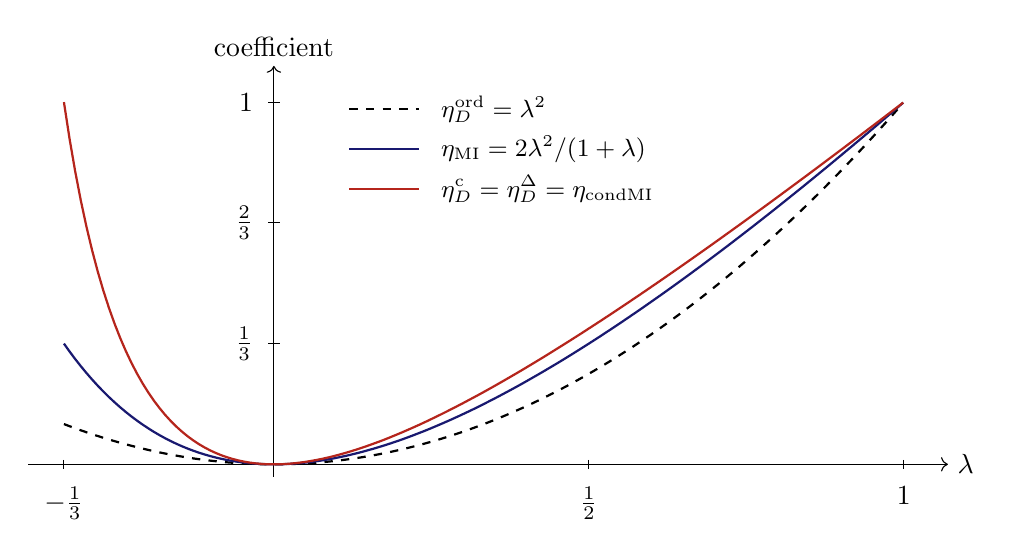
\begin{tikzpicture}[x=8cm,y=4.6cm]
 \draw[->] (-.39,0)--(1.07,0) node[right] {$\lambda$};
 \draw[->] (0,-.035)--(0,1.1) node[above] {coefficient};
 \foreach \x/\lab in {-.333333/{-\tfrac13},.5/{\tfrac12},1/{1}}{
   \draw (\x,.012)--(\x,-.012) node[below=3pt] {$\lab$};}
 \foreach \y/\lab in {.333333/{\tfrac13},.666667/{\tfrac23},1/{1}}{
   \draw (.009,\y)--(-.009,\y) node[left=2pt] {$\lab$};}
 \draw[thick,dashed,black,domain=-.333333:1,samples=150]
   plot (\x,{\x*\x});
 \draw[thick,MidnightBlue,domain=-.333333:1,samples=150]
   plot (\x,{2*\x*\x/(1+\x)});
 \draw[thick,BrickRed,domain=-.333333:1,samples=150]
   plot (\x,{3*\x*\x/(1+2*\x)});
 \draw[black,dashed,thick] (.12,.98)--(.23,.98);
 \node[anchor=west,font=\small] at (.25,.98) {$\eta_D^{\mathrm{ord}}=\lambda^2$};
 \draw[MidnightBlue,thick] (.12,.87)--(.23,.87);
 \node[anchor=west,font=\small] at (.25,.87) {$\eta_{\mathrm{MI}}=2\lambda^2/(1+\lambda)$};
 \draw[BrickRed,thick] (.12,.76)--(.23,.76);
 \node[anchor=west,font=\small] at (.25,.76) {$\eta_D^{\mathrm c}=\eta_D^\Delta
       =\eta_{\mathrm{condMI}}$};
\end{tikzpicture}
\caption{Three distinct qubit depolarizing contraction coefficients over the
full CP interval. At $\lambda=1/2$ their values are $1/4,1/3,3/8$.
At $\lambda=-1/3$ they are $1/9,1/3,1$.}
\label{fig:coefficients}
\end{figure}
% End sections/09-examples

% Begin sections/10-noise
\section{Orthogonal-unitary noise and a scoped mixing application}
\label{sec:noise}

For a specified error basis, the finite Choi optimization becomes a scalar
inverse-probability formula. Its dependence on rare errors explains why short
noise words and spectral gaps answer different quantitative questions.

\begin{theorem}[Orthogonal-unitary inverse probabilities]
\label{thm:error-basis}
Let $\{U_g:g=1,\ldots,d^2\}$ be an orthogonal unitary basis,
$\Tr U_g^*U_h=d\delta_{gh}$, and let
$\N_p(X)=\sum_g p_gU_gXU_g^*$.
If all probabilities are positive,
\begin{equation}
 M(\N_p)=\frac1{d^4}\sum_g\frac1{p_g},\qquad
 \beta(\N_p)=\frac{d^4}{\sum_g p_g^{-1}}.
 \label{eq:unitary-noise}
\end{equation}
If a probability is zero, $M=\infty$ and $\beta=0$.
\end{theorem}
\begin{proof}
The normalized vectors
$\ket{u_g}=\ket{U_g}\!\rangle/\sqrt d$ form an orthonormal
maximally entangled basis, and
$J=d\sum_g p_g\ket{u_g}\bra{u_g}$.
When all $p_g>0$,
\[
 \Tr_AJ^{-1}=\Tr_BJ^{-1}=cI_d,\qquad
 c=d^{-2}\sum_g p_g^{-1}.
\]
For every density $\sigma$, its positive inverse form $T_\sigma$
satisfies
\[
 \norm{T_\sigma}_\infty
 \geq\frac{\Tr T_\sigma}{d}
 =\frac cd\Tr\sigma^2\geq\frac c{d^2}.
\]
The center $I_d/d$ attains both inequalities, proving
\eqref{eq:unitary-noise}. If $p_g=0$, feasibility would force
$(I\otimes\sigma)\ket{u_g}=0$. Full Schmidt rank forces
$\sigma=0$, which is not a density.
\end{proof}

\begin{theorem}[Shortest-word onset for a fixed Weyl noise family]
\label{thm:word-onset}
Let the orthogonal basis be a projective Weyl representation of a
finite label group $G$, $|G|=d^2$, and consider
\[
 \mathcal L=\sum_{s\in S}\gamma_s(\Ad U_s-\id),\qquad
 T_t=e^{t\mathcal L},\qquad \gamma_s>0.
\]
Suppose $S$ generates $G$. Let $\ell(g)$ be the shortest directed
word length reaching $g$, put $r=\max_g\ell(g)$, and set
\[
 c_e=1,\qquad
 c_g=\frac1{\ell(g)!}
       \sum_{s_1\cdots s_{\ell(g)}=g}
                    \prod_{j=1}^{\ell(g)}\gamma_{s_j}\quad(g\ne e).
\]
At fixed group and fixed rates, as $t\downarrow0$,
\begin{equation}
 \beta(T_t)=
 \frac{d^4}{\sum_{\ell(g)=r}c_g^{-1}}\,t^r+O(t^{r+1}).
 \label{eq:word-onset}
\end{equation}
If the jumps generate only a proper subgroup, $\beta(T_t)=0$ for
every finite $t>0$. Given unit-cost group operations, all shortest
lengths and their leading coefficients require
$O(|G||S|)$ arithmetic operations.
\end{theorem}
\begin{proof}
Put $\Gamma=\sum_s\gamma_s$. The compound-Poisson expansion is
\[
 p_t(g)=e^{-\Gamma t}
 \sum_{k\geq0}\frac{t^k}{k!}
     \sum_{s_1\cdots s_k=g}\prod_{j=1}^k\gamma_{s_j}.
\]
Projective phases disappear under conjugation. For each fixed $g$,
$p_t(g)=c_gt^{\ell(g)}+O(t^{\ell(g)+1})$.
Substitute into \eqref{eq:unitary-noise}; the reciprocal sum is
dominated by all labels at maximal distance $r$. Inverting that
finite positive leading sum proves \eqref{eq:word-onset}.
If a label is unreachable, its probability is zero at all finite
times and \cref{thm:error-basis} applies.

Breadth-first search gives the directed lengths. On the resulting
acyclic shortest-path levels, sum products of rates over the
predecessors to obtain the shortest-word weights, then divide at
level $k$ by $k!$. Each edge is used a bounded number of times.
This proves the stated arithmetic count; it is not a bound uniform
in dimension or a claim about acquisition of the rates.
\end{proof}

For $n$ qubits the full error basis has $4^n$ labels. The finite-group
algorithm is therefore not polynomial in the qubit count. The asymptotic
remainder in \eqref{eq:word-onset} also concerns a fixed family; it
cannot be used without control when $G$ changes with $n$.

\subsection{Two independent Pauli errors}

For one qubit with $X$ and $Z$ jumps at rates $a,b>0$, the two parity
bits are independent, with odd probabilities
$(1-e^{-2at})/2$ and $(1-e^{-2bt})/2$.
Factoring their inverse-probability sum gives the exact identities
\begin{equation}
 \beta(T_t)=(1-e^{-4at})(1-e^{-4bt}),\qquad
 \alpha_+(T_t)=(1-e^{-2at})(1-e^{-2bt}).
 \label{eq:xz-exact}
\end{equation}
The second follows from $\alpha_+=4\min_g p_t(g)$, as proved in
\cref{thm:doeblin-comparison}.
In particular $\beta(T_t)=16ab\,t^2+O(t^3)$.
The nonidentity Pauli eigenoperators have generator eigenvalues
$-2a,-2b,-2(a+b)$, so the spectral gap is $2\min(a,b)>0$.
Nevertheless
\[
 \lim_{t\downarrow0}\frac{-\log\eta(T_t)}t=0.
\]
There is no $\kappa>0$ with $\eta(T_t)\leq e^{-\kappa t}$
uniformly from time zero. This is an all-pairs reference-assisted
statement and is compatible with positive fixed-equilibrium entropy
rates in other inequalities~\cite{GR22}.

\subsection{An exact tensor-product transition}

For $n$ independent qubits with equal $X,Z$ rates $\gamma>0$,
\cref{thm:products} and \eqref{eq:xz-exact} give, at every $t\geq0$,
\begin{align}
 \eta_n(t)&=1-(1-e^{-4\gamma t})^{2n}, \label{eq:noise-cutoff}\\
 T_n(\epsilon)
 &= -\frac1{4\gamma}
       \log\!\left[1-(1-\epsilon)^{1/(2n)}\right],
 \qquad 0<\epsilon<1. \label{eq:noise-threshold}
\end{align}
Here $T_n(\epsilon)$ is the first time $\eta_n(t)\leq\epsilon$.
At $t=(\log(2n)+c)/(4\gamma)$,
\[
 \eta_n(t)\longrightarrow 1-\exp(-e^{-c}).
\]
These follow directly by solving the scalar equation and taking
$(1-e^{-c}/(2n))^{2n}\to e^{-e^{-c}}$.

The positive CP-replacer bound
$\eta_n(t)\leq1-\alpha_{+,n}(t)$ uses
$\alpha_{+,n}(t)=(1-e^{-2\gamma t})^{2n}$.
For a fixed threshold it reaches its transition near
$\log(2n)/(2\gamma)$, whereas \eqref{eq:noise-threshold} has center
$\log(2n)/(4\gamma)$. This factor-two comparison is to that specific
Doeblin bound. Tensor-product quantum mixing cutoffs and the limitations
of spectral-gap estimates are established in \cite{KRW12}; we claim
neither a new general cutoff theorem nor superiority over every
available mixing method.
% End sections/10-noise

% Begin sections/11-acquisition
\section{Discontinuity and the obstruction to uniform acquisition}
\label{sec:acquisition}

An exact finite formula does not imply that its value is uniformly learnable
from experiments on an unknown channel. The support condition makes this
distinction sharp, even for one qubit.

\begin{theorem}[Jump at pure reset]
\label{thm:reset-jump}
Let $\mathcal A_\gamma$ be qubit amplitude damping with Kraus operators
\[
 K_0=\diag(1,\sqrt{1-\gamma}),\qquad
 K_1=\sqrt\gamma\,\ket0\bra1,\qquad 0\leq\gamma\leq1.
\]
For every $0\leq\gamma<1$, its complete and conditional Umegaki
coefficients and its conditional-MI coefficient are one. The analogous
three coefficients for every divergence in
\cref{thm:petz,thm:renyi-chernoff} are also one. At $\gamma=1$ all these
coefficients are zero. Nevertheless,
\begin{equation}
 \norm{\mathcal A_\gamma-\mathcal A_1}_\diamond
 \leq2\sqrt{2(1-\sqrt\gamma)}\longrightarrow0.
 \label{eq:reset-diamond}
\end{equation}
\end{theorem}
\begin{proof}
There is a direct coherent witness, independent of solving the Choi
optimization. In \eqref{eq:coherent-family} take
$R_0=\mathbb C$, $C=\diag(1-r,r)$, $0<r<1$,
$B=\ket1\bra0$ and $\tau=I_2/2$. Then $\Tr B=0$ and
$q_C(B)=1/r$. Writing $s=1-\gamma>0$ gives
\[
 C'=\diag(1-sr,sr),\qquad B'=\sqrt s\,\ket1\bra0,
 \qquad q_{C'}(B')=1/r.
\]
The coherent states are positive when $h^2<r/2$, independently of
their rare-sector weight, and both marginals are exactly fixed.
For Umegaki entropy their input and output Hessians are
\[
 2pq\,L(qr,p/2),\qquad
 2pqs\,L(qsr,p(1+\gamma)/2),
 \quad L(a,b)=\frac{\log a-\log b}{a-b}.
\]
Both, divided by $2p\log(1/p)$, tend to $1/r$.
The ordered perturbation and rare-sector limits thus give ratio one.
The uniform bit of \cref{sec:converse} gives the same CMI ratio.
For regular Petz and logarithmic divergences,
\cref{lem:petz-hessian,lem:chernoff-local} give the same ratio from
the two equal rectangular forms. Data processing bounds each
coefficient above by one; the conditional numerator is at most its
input counterpart by subtraction. Thus all these values are exactly
one. At $\gamma=1$ the channel is the pure replacer, so every output
divergence equals the reference divergence and each coefficient is zero.

For the norm bound use a common environment and isometries
\[
 V_\gamma\ket0=\ket{00},\qquad
 V_\gamma\ket1=\sqrt{1-\gamma}\ket{10}
                          +\sqrt\gamma\ket{01}.
\]
Their difference vanishes on $\ket0$ and has squared norm
$2(1-\sqrt\gamma)$ on $\ket1$.
For pure inputs with any reference, trace distance of the two
isometric outputs is at most twice their vector distance.
Convexity and partial-trace contractivity give
$\norm{\mathcal A_\gamma-\mathcal A_1}_\diamond
\leq2\norm{V_\gamma-V_1}$, proving
\eqref{eq:reset-diamond}.
\end{proof}

The lower witness uses a shrinking perturbation and a rare reference sector.
Its ratio remains close to one while its absolute information becomes
arbitrarily small. The theorem does not supply a finite communication rate
near complete damping.

\begin{theorem}[No uniformly bounded-use estimator]
\label{thm:no-uniform-estimator}
Fix $0<\epsilon<1/2$. There is no estimator that, for every unknown
qubit channel, estimates its complete Umegaki coefficient to additive
error $\epsilon$ with probability at least $2/3$, while using at most
a uniformly bounded number of channel calls.

The access model permits arbitrary finite ancillas, entangled inputs,
adaptive CPTP processing, intermediate measurements and classical
feedforward, and a final measurement. Calls are ordinary uses of the
unknown CPTP map. Access to a chosen dilation, its inverse, or a
controlled oracle is not provided.
The same impossibility holds for each of the other fixed coefficients
in \cref{thm:reset-jump}.
\end{theorem}
\begin{proof}
Suppose the worst-case call bound is $N$. Pad protocols with fewer
calls by ignored calls if needed. For two channels, replace one call
at a time in the $N$-round adaptive protocol. At each replacement
the trace norm changes by at most their diamond-norm distance;
subsequent CPTP processing cannot increase it. Thus the final
states have trace distance, with the factor $1/2$ convention, at most
\[
 \frac N2\norm{\mathcal A_\gamma-\mathcal A_1}_\diamond .
\]
Intermediate instruments and classical records are part of the
retained system, so this argument includes adaptive strategies.
Any final measurement has total-variation distance at most this value.

The exact coefficients are one for $\gamma<1$ and zero for $\gamma=1$.
Because $\epsilon<1/2$, thresholding a successful estimate at $1/2$
distinguishes these channels with success at least $2/3$ under either
hypothesis. The event that the estimate exceeds $1/2$ must therefore
have probabilities differing by at least $1/3$.
Choose $\gamma<1$ sufficiently close to one that the displayed
distance is smaller than $1/3$, using \eqref{eq:reset-diamond}.
This contradiction proves the theorem, including $N=0$.
\end{proof}

This is an information-access obstruction, independent of computational
power. It does not preclude evaluation from exact supplied Choi entries,
or an acquisition theorem under explicit support and spectral-margin
promises. It also does not preclude a pointwise procedure whose required
number of calls diverges near the discontinuity.
% End sections/11-acquisition

% Begin sections/12-discussion
\section{Scope and further questions}
\label{sec:discussion}

The main operation established here is exact evaluation of a specified
reference-assisted contraction problem from a finite channel description.
The complete and reference-subtracted Umegaki coefficients are equal
for every finite channel, and their value is the finite Choi program.
The explicit conditional-MI proof uses a separate conditioning memory.
For depolarizing channels the ordinary-MI coefficient is strictly smaller
at every nonconstant, nonidentity parameter, with an exact value for
qubits and proved bounds in higher dimension. These conclusions answer
the two comparisons posed for depolarization in
\cite[Section~3.3, equation~(3.66)]{HGNW26}: the first is equality,
and the second is strict away from the two trivial parameters.
They do not compute ordinary MI for an arbitrary channel.

The program has a block constraint of order $2dm$, an $m\times m$
density variable, and a Hermitian $dm\times dm$ auxiliary variable.
It eliminates unbounded reference dimension from evaluation.
This is a dense matrix input statement. It does not bypass the cost
of obtaining Choi entries from a circuit, a many-body description or
experiments. Nor is a finite SDP an assertion of uniformly conditioned
or strongly polynomial numerical evaluation. Exact support decisions
and the difference between strict feasibility and a nearby singular
channel remain consequential.

The regular modular Petz extension has finite endpoint value and recession
slope as genuine hypotheses. Fixed interior Petz R\'enyi orders and
Chernoff divergence require their own logarithmic and optimization
arguments. No assertion has been made for sandwiched, maximal or
hockey-stick divergences, or for general orders above one. The reference
dimensions bound the witnesses needed for a supremum; they give neither
a lower bound on the information in those witnesses nor a uniform
precision requirement for constructing them.

The signed lift reconstructs observable means with weighted-square
control. It is not required to preserve positive observables, and it
has not been converted into a physical postprocessing channel.
In particular the scalar self-coefficient alone supplies no comparison
between a receiver and its complement. Capacity and recovery conclusions
would require additional channel-order hypotheses, of the kind studied
in \cite{ZW26v3,Hirche26}.

Several precise questions remain. What support and spectral promises
make acquisition from noisy channel data stable with useful costs?
What remains of exact sharpness when absolute input information and
preparation precision are constrained? Can the exact ordinary-MI
coefficient be found in dimension greater than two? For which additional
divergences does the positive-center erasure comparison give the sharp
linear coefficient? General noncommuting noise-onset prefactors and
succinct-generator complexity involve further structures beyond the
fixed-Weyl application proved here.

The distinction between exact evaluation, robust acquisition and a useful
physical protocol is therefore retained throughout. Each is a separate
mathematical operation.
% End sections/12-discussion

\Needspace{8\baselineskip}
\section*{Acknowledgements and AI use}
\addcontentsline{toc}{section}{Acknowledgements and AI use}
The mathematical ideas, constructions, proofs, and manuscript were developed by
GPT-6 Astra, with additional AI assistance for review. Human input was minimal and
consisted primarily of setting the research objectives and providing occasional
feedback.
\appendix
% Begin sections/appendix-classical
\section{The ordinary symmetric classical coefficient}
\label{app:classical}

This appendix proves \eqref{eq:symmetric-classical} independently of
the reference-assisted theorem. Let $k\geq2$, $a\geq0$, $b>0$ and
$a+(k-1)b=1$, and put $c=a-b$. For an interior probability vector
$p$ and a real tangent $v$ with $\sum_i v_i=0$, the input and output
KL Hessians are
\[
 \sum_i\frac{v_i^2}{p_i},\qquad
 c^2\sum_i\frac{v_i^2}{b+cp_i}.
\]
If $c=0$ the channel is constant. Otherwise it suffices to prove
\begin{equation}
 \sum_i d_i v_i^2\geq0,\qquad
 d_i=\frac1{p_i}-\frac{a+b}{b+cp_i}
     =\frac{b(1-2p_i)}{p_i(b+cp_i)}.
 \label{eq:classical-fisher}
\end{equation}
All denominators are positive at an interior prior, including when $a=0$.
If every $p_i\leq1/2$, each summand is nonnegative.
Otherwise exactly one coordinate, call it $p_0$, exceeds $1/2$.
Put $q=1-p_0<1/2$. For the other coordinates $d_i>0$, and weighted
Cauchy--Schwarz gives
\[
 \sum_{i\ne0}d_i v_i^2
 \geq \frac{v_0^2}{\sum_{i\ne0}d_i^{-1}} .
\]
For $0<t<1/2$, set
$h(t)=t(b+ct)/[b(1-2t)]$.
The function $h(t)/t$ is increasing, because its derivative is
$(a+b)/[b(1-2t)^2]>0$.
Consequently
\[
 \sum_{i\ne0}d_i^{-1}=\sum_{i\ne0}h(p_i)\leq h(q).
\]
Moreover $h(q)\leq-1/d_0$. Indeed, after multiplying by the common
positive denominator $b(2p_0-1)$, this is
$q(b+cq)\leq p_0(b+cp_0)$; the difference is
$(2p_0-1)(b+c)=(2p_0-1)a\geq0$.
Thus the last weighted sum is at least $-d_0v_0^2$,
proving \eqref{eq:classical-fisher}.

Integrate the Hessian comparison along the segment between two
positive distributions to obtain the KL upper bound
$c^2/(a+b)$. Common faithful regularization and
\cref{lem:entropy-integration} extend it to all finite-KL pairs.
For sharpness, use the prior placing probability $1/2$ on each of two
symbols and perturb those two probabilities oppositely.
The two relevant output probabilities are both $(a+b)/2$.
Its Hessian ratio is exactly $c^2/(a+b)$, and the finite-pair ratios
approach it. This proves \eqref{eq:symmetric-classical}, including
the exclusion case $a=0$.

For the associated measure-and-prepare quantum channel, its ordinary
unreferenced quantum coefficient has the same value. Dephasing the
input pair cannot increase relative entropy; applying the stochastic
channel then gives the classical upper bound. Diagonal input pairs
give the reverse bound.
% End sections/appendix-classical

% Begin sections/appendix-metrics
\section{Information identities and metric facts}
\label{app:metrics}

\subsection{Product-reference contraction equals ordinary MI contraction}
\label{app:product-mi}

We prove the identity used in \cref{prop:hierarchy}, with credit to the
corresponding result in \cite[Corollary~3]{HGNW26}.
Put $\kappa=\etaMI(\N)$. First $\etaOrd\leq\kappa$.
Given a finite-relative-entropy pair $\rho,\sigma$, a classical bit
selects $\rho$ with probability $a$ and $\sigma$ with probability
$1-a$. Its average is $\mu_a=a\rho+(1-a)\sigma$, and
\[
 I(U;A)=aD(\rho\|\mu_a)+(1-a)D(\sigma\|\mu_a).
\]
On $\supp\sigma$, the state $\sigma$ is faithful and $\rho$ is
supported there. As $a\downarrow0$,
$D(\rho\|\mu_a)\to D(\rho\|\sigma)$ and
$D(\sigma\|\mu_a)=O(a^2)$.
The first assertion uses continuity of the logarithm on that support;
the second is its Taylor expansion with zero first derivative.
The identical assertions hold after the channel on $\supp\N(\sigma)$.
Therefore the MI ratio tends to the relative-entropy ratio, proving
$\etaOrd\leq\kappa$.

For any product-reference comparison with finite input entropy,
\[
 D(\rho_{RA}\|\rho_R\otimes\sigma_A)
 =I(R;A)_\rho+D(\rho_A\|\sigma_A).
\]
At the output the two terms contract by at most $\kappa$ and
$\etaOrd$, respectively. Thus their sum contracts by at most
$\kappa$, proving $\etaP\leq\kappa$.
If the input MI is zero its output MI is also zero, since the state
is a product, so this argument includes zero-information summands.
Choosing $\sigma_A=\rho_A$ gives the reverse inequality
$\etaP\geq\kappa$.
Finally these product-reference pairs have the same reference marginal,
so $\etaP\leq\etaC$. Together with \cref{thm:main} this proves
\eqref{eq:hierarchy}.

\subsection{Joint convexity from the metric representation}
\label{app:metric-convexity}

For faithful $\omega$ and Hermitian $H$, each integrand in
\eqref{eq:bkm} is jointly convex in $(\omega,H)$.
Indeed, by inverse quadratic duality it is the supremum over $Y$ of
\[
 2\Rea\Tr Y^*H-\Tr Y^*[(1-u)L_\omega+uR_\omega]Y,
\]
which is affine in that pair. Integration proves joint convexity of
$g_\omega(H)$. The affine-path formula
\eqref{eq:entropy-integral} then proves joint convexity of
$D(\rho\|\sigma)$ for faithful pairs. For pairs with finite relative
entropy, mix every state with the same faithful state and apply
\cref{lem:entropy-integration}. If a positive-weight term on the
right is infinite, the inequality is automatic.
This proves precisely the convexity used in
\cref{thm:qubit-mi}, including the required boundary cases.

For binary pinching there is also a direct coherence proof. Write
$\Delta=(\id+\Ad Z)/2$ with $Z^2=I$, and set
$\sigma=\Delta\rho$, $H=\rho-\sigma$.
For faithful $\rho$, the function
$t\mapsto g_{\sigma+tH}(H)$ is convex by the preceding argument and
even because $Z\sigma Z=\sigma$, $ZHZ=-H$.
It is therefore nondecreasing for $0\leq t\leq1$.
For $0\leq\theta\leq1$, the affine-path formula gives
\[
 D(\sigma+\theta H\|\sigma)
 =\theta^2\int_0^1(1-s)g_{\sigma+\theta sH}(H)\dd s
 \leq\theta^2D(\rho\|\Delta\rho).
\]
For negative $\theta$, conjugation by $Z$ reduces the assertion to
$|\theta|$. Common faithful regularization and the entropy identity
$D(\rho\|\Delta\rho)=S(\Delta\rho)-S(\rho)$ handle arbitrary states.
This is an independent check of the two-sector case of
\cref{lem:twirl-coherence}.

\subsection{Ordinary qubit depolarizing contraction}
\label{app:ordinary-qubit}

Represent a qubit state by
$\rho=(I+\mathbf r\cdot\boldsymbol\sigma)/2$, $r=|\mathbf r|<1$.
On the trace-one affine space the entropy potential is
\[
 F(r)=\frac{1+r}{2}\log\frac{1+r}{2}
      +\frac{1-r}{2}\log\frac{1-r}{2}.
\]
For a tangent $H=(\mathbf v\cdot\boldsymbol\sigma)/2$, decompose
$\mathbf v$ into components parallel and perpendicular to
$\mathbf r$. Differentiating this radial function gives
\[
 g_\rho(H)=
 \frac{|\mathbf v_\parallel|^2}{1-r^2}
 +\frac{\operatorname{arctanh}r}{r}|\mathbf v_\perp|^2.
\]
At $r=0$ both coefficients have limit one.
Each coefficient is nondecreasing in $r$:
for the second use
$\operatorname{arctanh}r/r=\sum_{j\geq0}r^{2j}/(2j+1)$.
Depolarization sends $(\mathbf r,\mathbf v)$ to
$(\lambda\mathbf r,\lambda\mathbf v)$.
For $|\lambda|\leq1$ it consequently contracts the metric by at most
$\lambda^2$. Integrating along the state segment and taking finite
relative-entropy boundary limits proves the ordinary upper bound.
Infinitesimal perturbations around $I_2/2$ attain the metric ratio
$\lambda^2$, proving equality. In particular the proof covers the
negative CP interval without any partial-transpose invariance claim.

This agrees with the ordinary contraction theory discussed in
\cite{HR15}; the purpose of the calculation is to make the three-way
comparison in \cref{fig:coefficients} self-contained.
% End sections/appendix-metrics

% Begin sections/appendix-boundaries
\section{Finite checks and an excluded higher-order extension}
\label{app:checks}

\subsection{A fully specified rational fixed-reference example}
\label{app:finite-witness}

The source package contains small exact-arithmetic checks of examples, not
a numerical substitute for the proofs above. Here is the fixed-reference
example in full.
Use ternary exclusion and a three-dimensional reference
$R=\mathbb C^2\oplus\mathbb C r$. Put
\[
 u_0=\binom{1/2}{0},\quad u_1=\binom0{1/2},\quad
 u_2=\binom{-1/2}{-1/2},\quad
 n=10000,\quad p=\frac1{1+n^2},\quad q=1-p,\quad t=\frac1{10}.
\]
For a uniform bit $U=\pm1$, define subnormalized reference blocks,
indexed by the classical input $x$, by
\[
 \rho_x^\pm=
 \begin{pmatrix}
 q u_xu_x^*&\pm t\sqrt{pq}\,u_x\\
 \pm t\sqrt{pq}\,u_x^*&p/3
 \end{pmatrix}.
\]
Every entry is rational since $\sqrt{pq}=n/(1+n^2)$.
The states have trace one after summing over $x$ because
$\sum_x\norm{u_x}^2=1$. On the support of $u_x$ their Schur
complements equal $p(1/3-t^2)>0$, proving positivity.
Since $\sum_xu_x=0$, the two reference marginals agree exactly;
their input probabilities also agree. Thus $I(U;R)=I(U;X)=0$.
Their average deletes the displayed off-diagonal blocks.
The output blocks of exclusion are
$\rho_y'=(\sum_x\rho_x-\rho_y)/2$.

The supplied rational-interval calculation encloses the resulting ratio by
\[
 0.918490786084546654
 <\frac{I(U;Y|R)}{I(U;X|R)}
 <0.918490786084547090,
\]
above the ordinary classical coefficient $1/2$.
The input information is between
$5.513760010993645\times10^{-9}$ and
$5.513760010993648\times10^{-9}$ nats.
This small signal is reported explicitly.

The certificate isolates the eigenvalues of the rational block matrices
using rational characteristic-polynomial intervals. To bound logarithms it
reduces to $1\leq z\leq2$ and uses, with $v=(z-1)/(z+1)$,
\[
 \log z=2\sum_{j=0}^{N-1}\frac{v^{2j+1}}{2j+1}+R_N,\qquad
 0\leq R_N\leq
 \frac{2v^{2N+1}}{(2N+1)(1-v^2)}.
\]
The remainder follows by bounding the positive tail termwise by a
geometric series. Integer-square-root enclosures are used in the
separate qubit-reference ternary example. All comparisons in these
checks use rational endpoints rounded outward, not floating-point
optimization.

The latter qubit-reference example has parameters
$p=1/10,s=1/100,h=1/100$ and states
\begin{align*}
 \rho_{XR}(p,s)
 &=\frac{1-p}{2}\ket0\bra0\otimes\ket{\psi_+}\bra{\psi_+}
 +\frac{1-p}{2}\ket1\bra1\otimes\ket{\psi_-}\bra{\psi_-}\\
 &\quad+p\ket2\bra2\otimes\ket1\bra1,\\
 \ket{\psi_\pm}&=\sqrt{1-s}\ket0\pm\sqrt s\ket1.
\end{align*}
A bit selects $p+h$ or $p-h$. Its conditional-information ratio lies
between $0.927420641599022566$ and $0.927420641599022567$.
Here the two reference marginals may differ; this example must not be
identified with the exactly fixed-reference construction above.

\subsection{An exact depolarizing quadratic check}

For $\lambda=1/2$ in dimension two, the matrix-unit Gram tuple with
center $a_i=(5/8)\Tr F_i/2$ has defect
\[
 \frac38\mathbf G-(\mathbf A-aI)(\mathbf A-aI)^*
\]
with eigenvalues $0$ twice, $3/32$ four times and $15/128$ twice.
Let $P_0$ be its kernel projection, $C=P_0/2$ and
$B=C(\mathbf A-aI)$. The included rational calculation verifies
$\Tr C=1$, $\Tr_A B=0$, and the range conditions for the two
quadratic forms. Their values are $q_C(B)=3/8$ and
$q_{C'}(B')=9/64$, with pseudoinverses on these particular singular
supports. Faithful mixtures of $C$ give the same limiting ratio.
The positive-center Choi calculation gives $M=8/5$.
These are exact finite checks of the value $3/8$; the universal
optimality proof is \cref{sec:gram}--\cref{sec:converse}.

\subsection{Why an all-order Petz R\'enyi claim is false}
\label{app:order-ten}

There is no extension of \eqref{eq:renyi-exact} to every order above
one. For qubit shrinkage $1/2$ use the diagonal pair
$P=(1,0)$, $Q=(9/10,1/10)$.
The input Petz order-ten divergence is $\log(10/9)$.
The output laws are $(3/4,1/4)$ and $(7/10,3/10)$, so its
output divergence is $(\log R)/9$, where the positive rational
\[
 R=\frac{(3/4)^{10}}{(7/10)^9}
   +\frac{(1/4)^{10}}{(3/10)^9}
\]
satisfies $R^8>(10/9)^{27}$ by direct integer arithmetic.
Hence the output-to-input ratio exceeds $3/8$.
The source package includes the short rational check of this inequality.
Order ten is outside the usual Petz data-processing range. This example
does not settle the different question of exact coefficients for
$1<\alpha\leq2$.
% End sections/appendix-boundaries

{\small\raggedright

\begin{thebibliography}{10}

\bibitem{ACM+07}
K.~M.~R. Audenaert, J.~Calsamiglia, Ll. Masanes, R.~Mu{\~n}oz-Tapia,
  A.~Ac{\'i}n, E.~Bagan, and F.~Verstraete.
\newblock The quantum {Chernoff} bound.
\newblock {\em Physical Review Letters}, 98:160501, 2007.
\newblock
  \href{https://doi.org/10.1103/PhysRevLett.98.160501}{doi:10.1103/PhysRevLett.98.160501}.

\bibitem{Balsu26}
Akshay Balsubramani.
\newblock All you need is log.
\newblock \href{https://arxiv.org/abs/2606.27349v3}{arXiv:2606.27349v3}, 2026.
\newblock Version 3, 24 September 2026.

\bibitem{Choi75}
Man-Duen Choi.
\newblock Completely positive linear maps on complex matrices.
\newblock {\em Linear Algebra and its Applications}, 10(3):285--290, 1975.
\newblock
  \href{https://doi.org/10.1016/0024-3795(75)90075-0}{doi:10.1016/0024-3795(75)90075-0}.

\bibitem{FH14}
Uwe Franz and Fumio Hiai.
\newblock Conic structure of the non-negative operator convex functions on
  $(0,\infty)$.
\newblock \href{https://arxiv.org/abs/1310.1539v2}{arXiv:1310.1539v2}, 2014.
\newblock Version 2, 16 May 2014.

\bibitem{GR22}
Li~Gao and Cambyse Rouz{\'e}.
\newblock Complete entropic inequalities for quantum {Markov} chains.
\newblock \href{https://arxiv.org/abs/2102.04146v3}{arXiv:2102.04146v3}, 2021.
\newblock Version 3, 14 June 2021.

\bibitem{GHNW26}
Ian George, Christoph Hirche, Theshani Nuradha, and Mark~M. Wilde.
\newblock Quantum {Doeblin} coefficients: Interpretations and applications.
\newblock {\em Quantum}, 10:2115, 2026.
\newblock
  \href{https://doi.org/10.22331/q-2026-05-22-2115}{doi:10.22331/q-2026-05-22-2115};
  \href{https://arxiv.org/abs/2503.22823v3}{arXiv:2503.22823v3}.

\bibitem{HR15}
Fumio Hiai and Mary~Beth Ruskai.
\newblock Contraction coefficients for noisy quantum channels.
\newblock \href{https://arxiv.org/abs/1508.03551}{arXiv:1508.03551}, 2015.

\bibitem{Hirche26}
Christoph Hirche.
\newblock Quantum estimation, channel orders, and private capacity.
\newblock \href{https://arxiv.org/abs/2610.03706v1}{arXiv:2610.03706v1}, 2026.
\newblock Version 1, 2 October 2026.

\bibitem{HGNW26}
Christoph Hirche, Ian George, Theshani Nuradha, and Mark~M. Wilde.
\newblock Conditional contraction coefficients and their applications to
  quantum networks.
\newblock \href{https://arxiv.org/abs/2608.27171v1}{arXiv:2608.27171v1}, 2026.
\newblock Version 1, 27 August 2026.

\bibitem{HT24}
Christoph Hirche and Marco Tomamichel.
\newblock Quantum {R\'enyi} and $f$-divergences from integral representations.
\newblock \href{https://arxiv.org/abs/2306.12343v3}{arXiv:2306.12343v3}, 2024.
\newblock Version 3, 26 August 2024.

\bibitem{KRW12}
Michael~J. Kastoryano, David Reeb, and Michael~M. Wolf.
\newblock A cutoff phenomenon for quantum {Markov} chains.
\newblock {\em Journal of Physics A: Mathematical and Theoretical},
  45(7):075307, 2012.
\newblock
  \href{https://doi.org/10.1088/1751-8113/45/7/075307}{doi:10.1088/1751-8113/45/7/075307}.

\bibitem{NS09}
Michael Nussbaum and Arleta Szko{\l}a.
\newblock The {Chernoff} lower bound for symmetric quantum hypothesis testing.
\newblock {\em The Annals of Statistics}, 37(2):1040--1057, 2009.
\newblock \href{https://doi.org/10.1214/08-AOS593}{doi:10.1214/08-AOS593}.

\bibitem{OP21}
Or~Ordentlich and Yury Polyanskiy.
\newblock Strong data processing constant is achieved by binary inputs.
\newblock \href{https://arxiv.org/abs/2010.01987v2}{arXiv:2010.01987v2}, 2021.
\newblock Version 2, 4 June 2021.

\bibitem{Petz86}
D{\'e}nes Petz.
\newblock Quasi-entropies for finite quantum systems.
\newblock {\em Reports on Mathematical Physics}, 23(1):57--65, 1986.
\newblock
  \href{https://doi.org/10.1016/0034-4877(86)90067-4}{doi:10.1016/0034-4877(86)90067-4}.

\bibitem{Sion58}
Maurice Sion.
\newblock On general minimax theorems.
\newblock {\em Pacific Journal of Mathematics}, 8(1):171--176, 1958.
\newblock
  \href{https://doi.org/10.2140/pjm.1958.8.171}{doi:10.2140/pjm.1958.8.171}.

\bibitem{Stinespring55}
W.~Forrest Stinespring.
\newblock Positive functions on {$C^*$}-algebras.
\newblock {\em Proceedings of the American Mathematical Society},
  6(2):211--216, 1955.
\newblock
  \href{https://doi.org/10.1090/S0002-9939-1955-0069403-4}{doi:10.1090/S0002-9939-1955-0069403-4}.

\bibitem{ZW26v3}
Chengkai Zhu and Xin Wang.
\newblock Quantum incapacity from observable shadows.
\newblock \href{https://arxiv.org/abs/2607.24693v3}{arXiv:2607.24693v3}, 2026.
\newblock Version 3, revised 5 October 2026.

\end{thebibliography}

}
\end{document}
